\section{Numerical Experiments}\label{sec:exp} 
In what follows, \Cref{sec:exp1} is themed around the key insight obtained from \Cref{th:main}, i.e., the correlation of the gates lies at the heart of `what is learnt in a DNN with ReLUs'. In particular, we show that operations (such as permuting the layers, shifting and rotating the gates, and giving a constant input to the value network) that destroy the layer by layer computational structure do not degrade test performance. These operations lead to combinatorially many models and in all of them the test performance remains the same. In \Cref{sec:exp2} we throw light on the open question in \citenum{randlabel} on why test performance degrades due to upstream training with random labels.
% Prior vs now what is the difference : robustness + random label etc
%Datasets are MNIST and CIFAR-10. For MNIST, we use the DGN in \Cref{fig:dgn-prior-new} (right) with fully connected layers instead of the convolutional layers.  All models are trained with `\emph{Adam}'  \cite{adam} (step-size $=3\cdot 10^{-4}$ , batch size $=32$). 
\subsection{Experiment 1: Destroying layer-by-layer structure does not affect performance}\label{sec:exp1}
The aim of the experiment is to investigate the information in the gates and to show that it is invariant even if we destroy the layer-by-layer structure. The gates themselves are basically of three kinds as described below.
$1.$ Fixed Learnt: We \emph{pre-train} the feature network (which is a DNN with ReLUs), then \emph{freeze} the weights of the feature network, and then train the value network. This way we can measure information in the gates of a trained DNN.\\
$2.$ Fixed Random: We initialise the feature network at random, and then \emph{freeze} its weights and then train the value network. This way we can measure information in the gates of a DNN at initialisation. Here, the feature and value network can be either initialised with the same weights (i.e., dependent initialisation) or statistically independent weights (i.e., independent initialisation).
$3.$ Decoupled Learning: We initialise the weights of the value and feature network statistically independent and then train both of them. For the gradient to flow through the feature network we use \emph{soft-gating}, i.e., $G(q)=\frac{1}{1+\exp{-\beta\cdot q}}$, with $\beta=10$. 




\textbf{Prior Work (4 Regimes, 1 Model Per Regime ).} 
Recall from \Cref{sec:dgn}, that a DGN consists of two distinct networks of identical architecture namely the feature network and the value network. Both the feature network and value network have $4$ convolutional layers $C1,\ldots,C4$ followed by a global average pooling (GAP) layer, a linear layer and a final `softmax' layer. $\hat{y}_{\text{DGN}}$ is the output of the DGN (performance is measured with respect to this output). $\hat{y}_{\text{f}}$ is used only when we want to \emph{pre-train} the feature network. The feature network has ReLUs, whereas the value network uses the gates from feature network as external masks. Here, $G_1,\ldots,G_4$ are the gates of layers $1,\ldots,4$ of feature network and in the prior setup these are used directly in the value network. The DGN has the following $\mathbf{4}$ {gating regimes} based on the initialisation and trainability of the feature network parameters. In all these regimes, the output of the DGN is $\hat{y}_{\text{DGN}}$. 

\quad 1. \emph{Fixed Random-Dependent Initialisation} (\textbf{FR-DI}): Both value network and feature network are initialised at random and identically, i.e., $\Tf_0=\Tv_0$. Only the value network is trained and the feature network is fixed, i.e., $\Tf_t=\Tf_0,\forall t\geq 0$.

\quad 2. \emph{Fixed Random-Independent Initialisation} (\textbf{FR-II}): Both value network and feature network are initialised at random and statistically independent of each other, i.e., $\Tf_0\perp \Tv_0$. Only the value network is trained and the feature network is fixed, i.e., $\Tf_t=\Tf_0,\forall t\geq 0$.

\quad 3. \emph{Fixed Learnt} (\textbf{FL}): The feature network is \textbf{pre-trained} first using $\hat{y}_{\text{f}}$ as output. Then the value network is initialised at random, and only the value network is trained and the feature network is fixed.

\quad 4. \emph{Decoupled learning} (\textbf{DL}): Both value and feature networks are initialised at random, and \textbf{both are trained}. In order to ensure that gradient flows through the feature network, we make use of \emph{soft-gating}, i.e., $G(q)=\frac{1}{1+\exp{-\beta\cdot q}}$, with $\beta=10$. 

\begin{figure}[h]
\centering
\begin{minipage}{0.49\columnwidth}
\centering
\resizebox{\columnwidth}{!}{
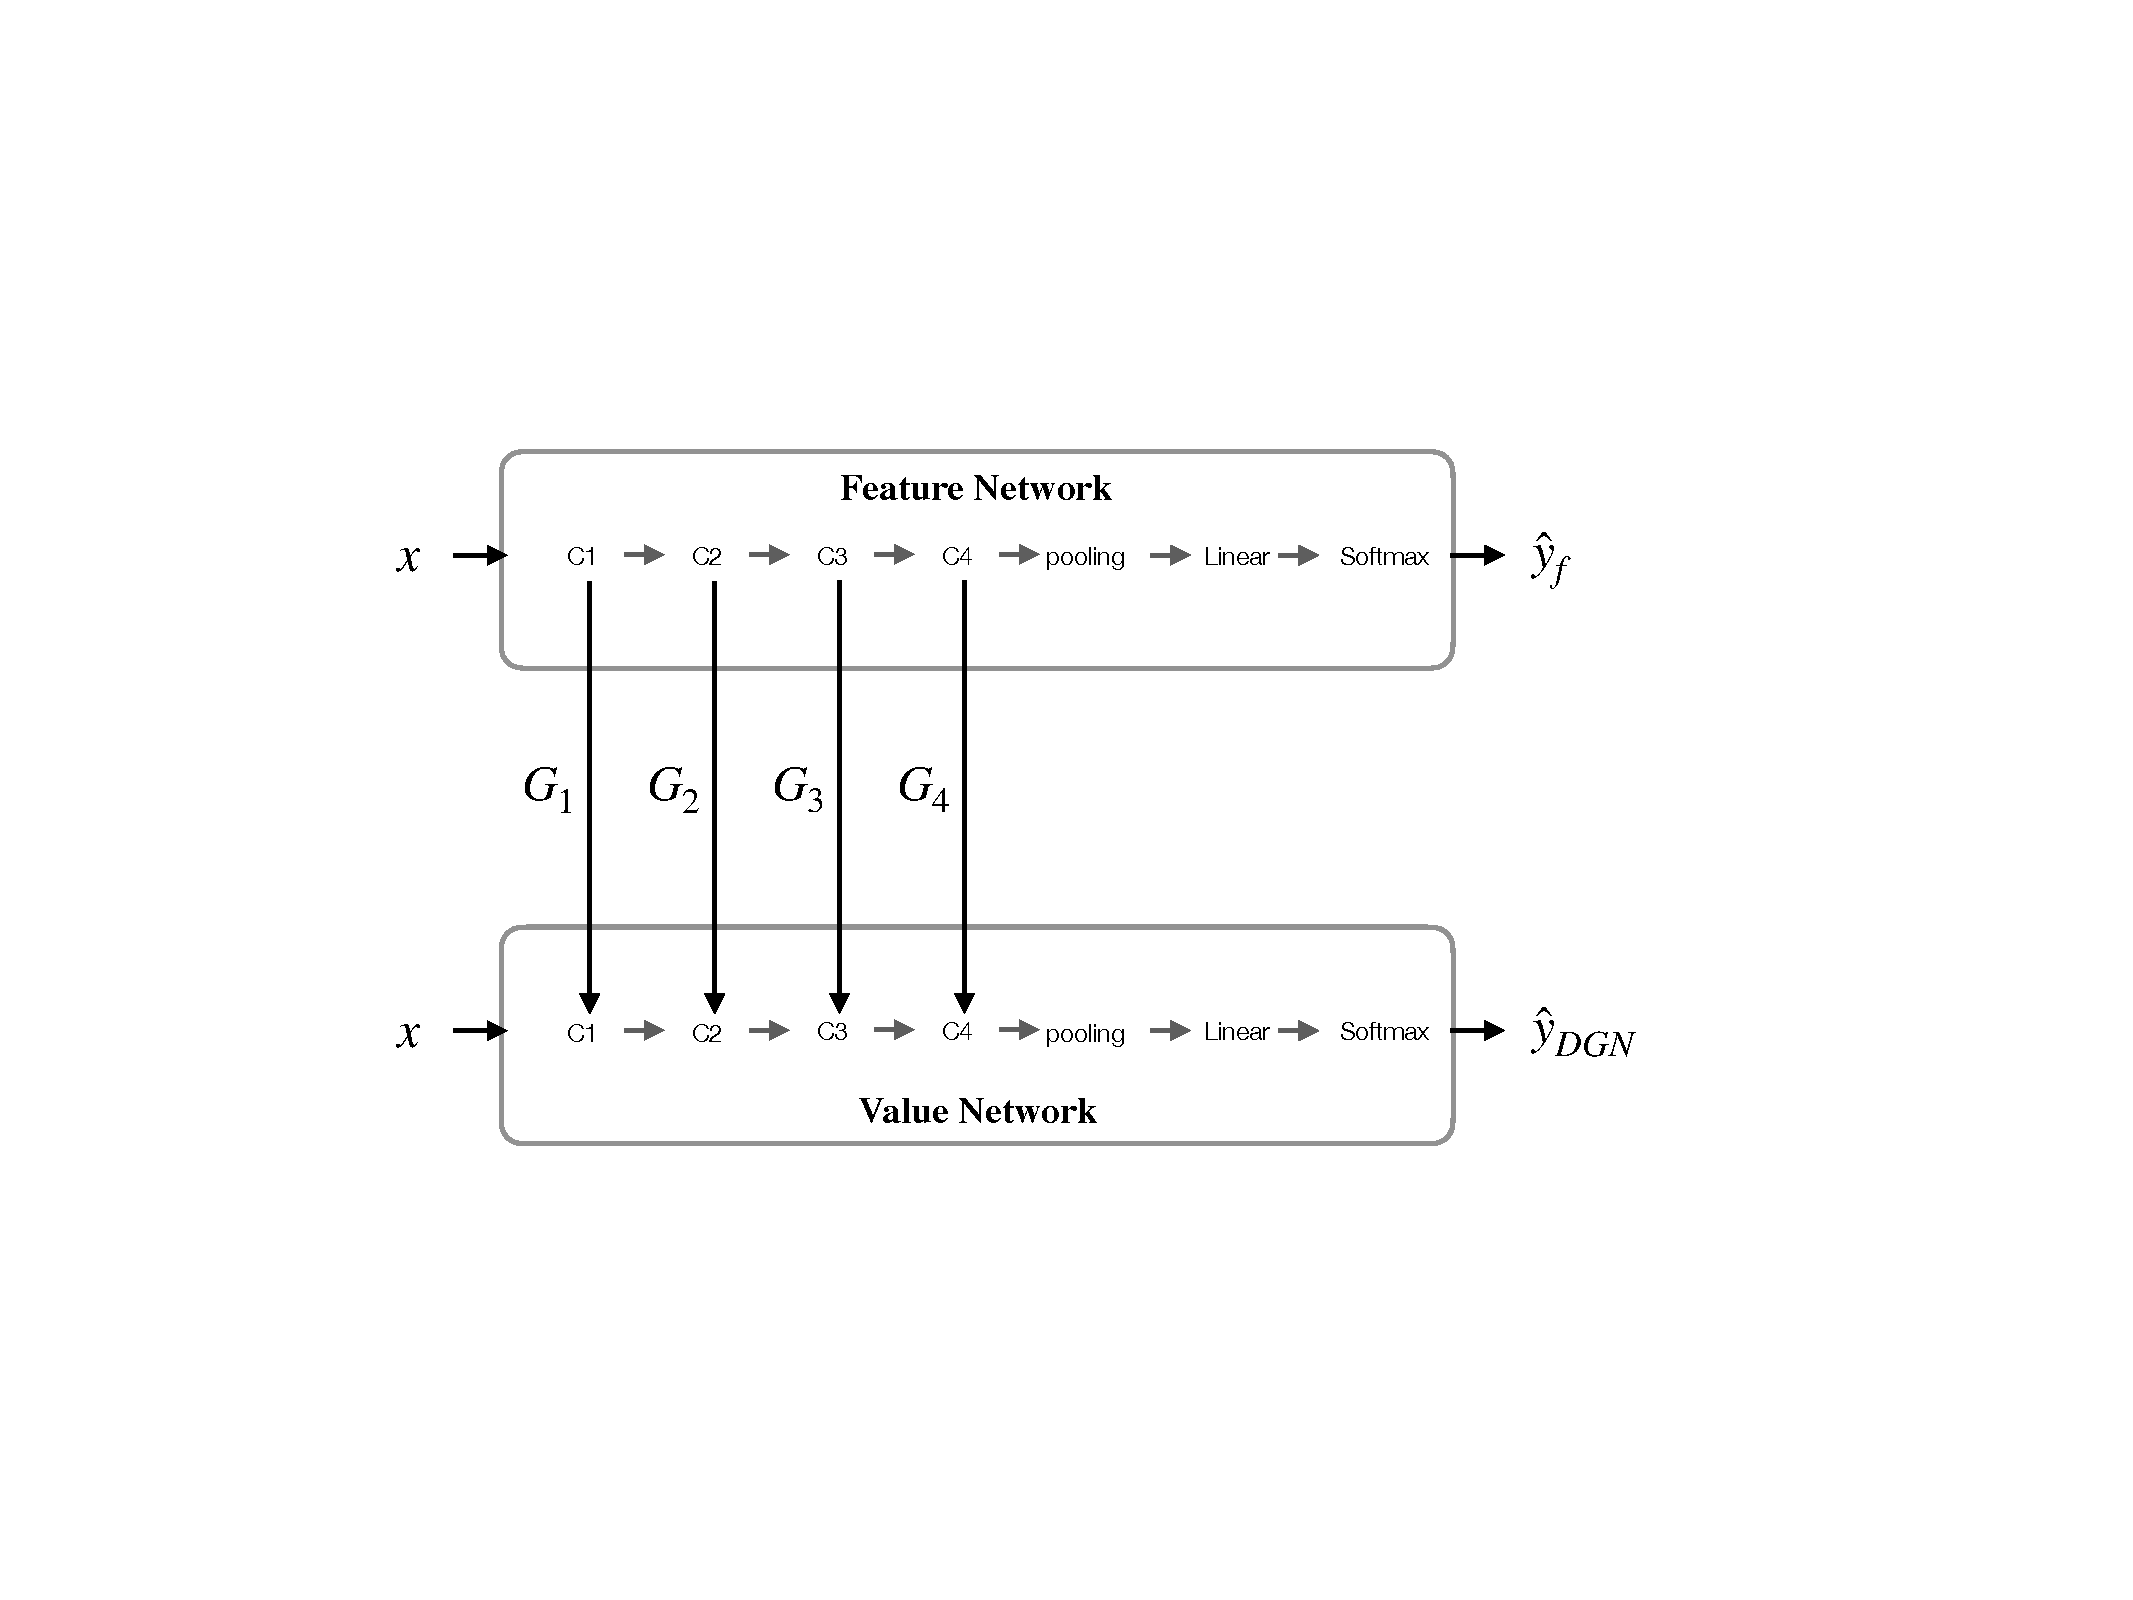
\includegraphics[scale=0.3]{figs/exp-prior.pdf}
}
\end{minipage}
\begin{minipage}{0.49\columnwidth}
\centering
\resizebox{\columnwidth}{!}{
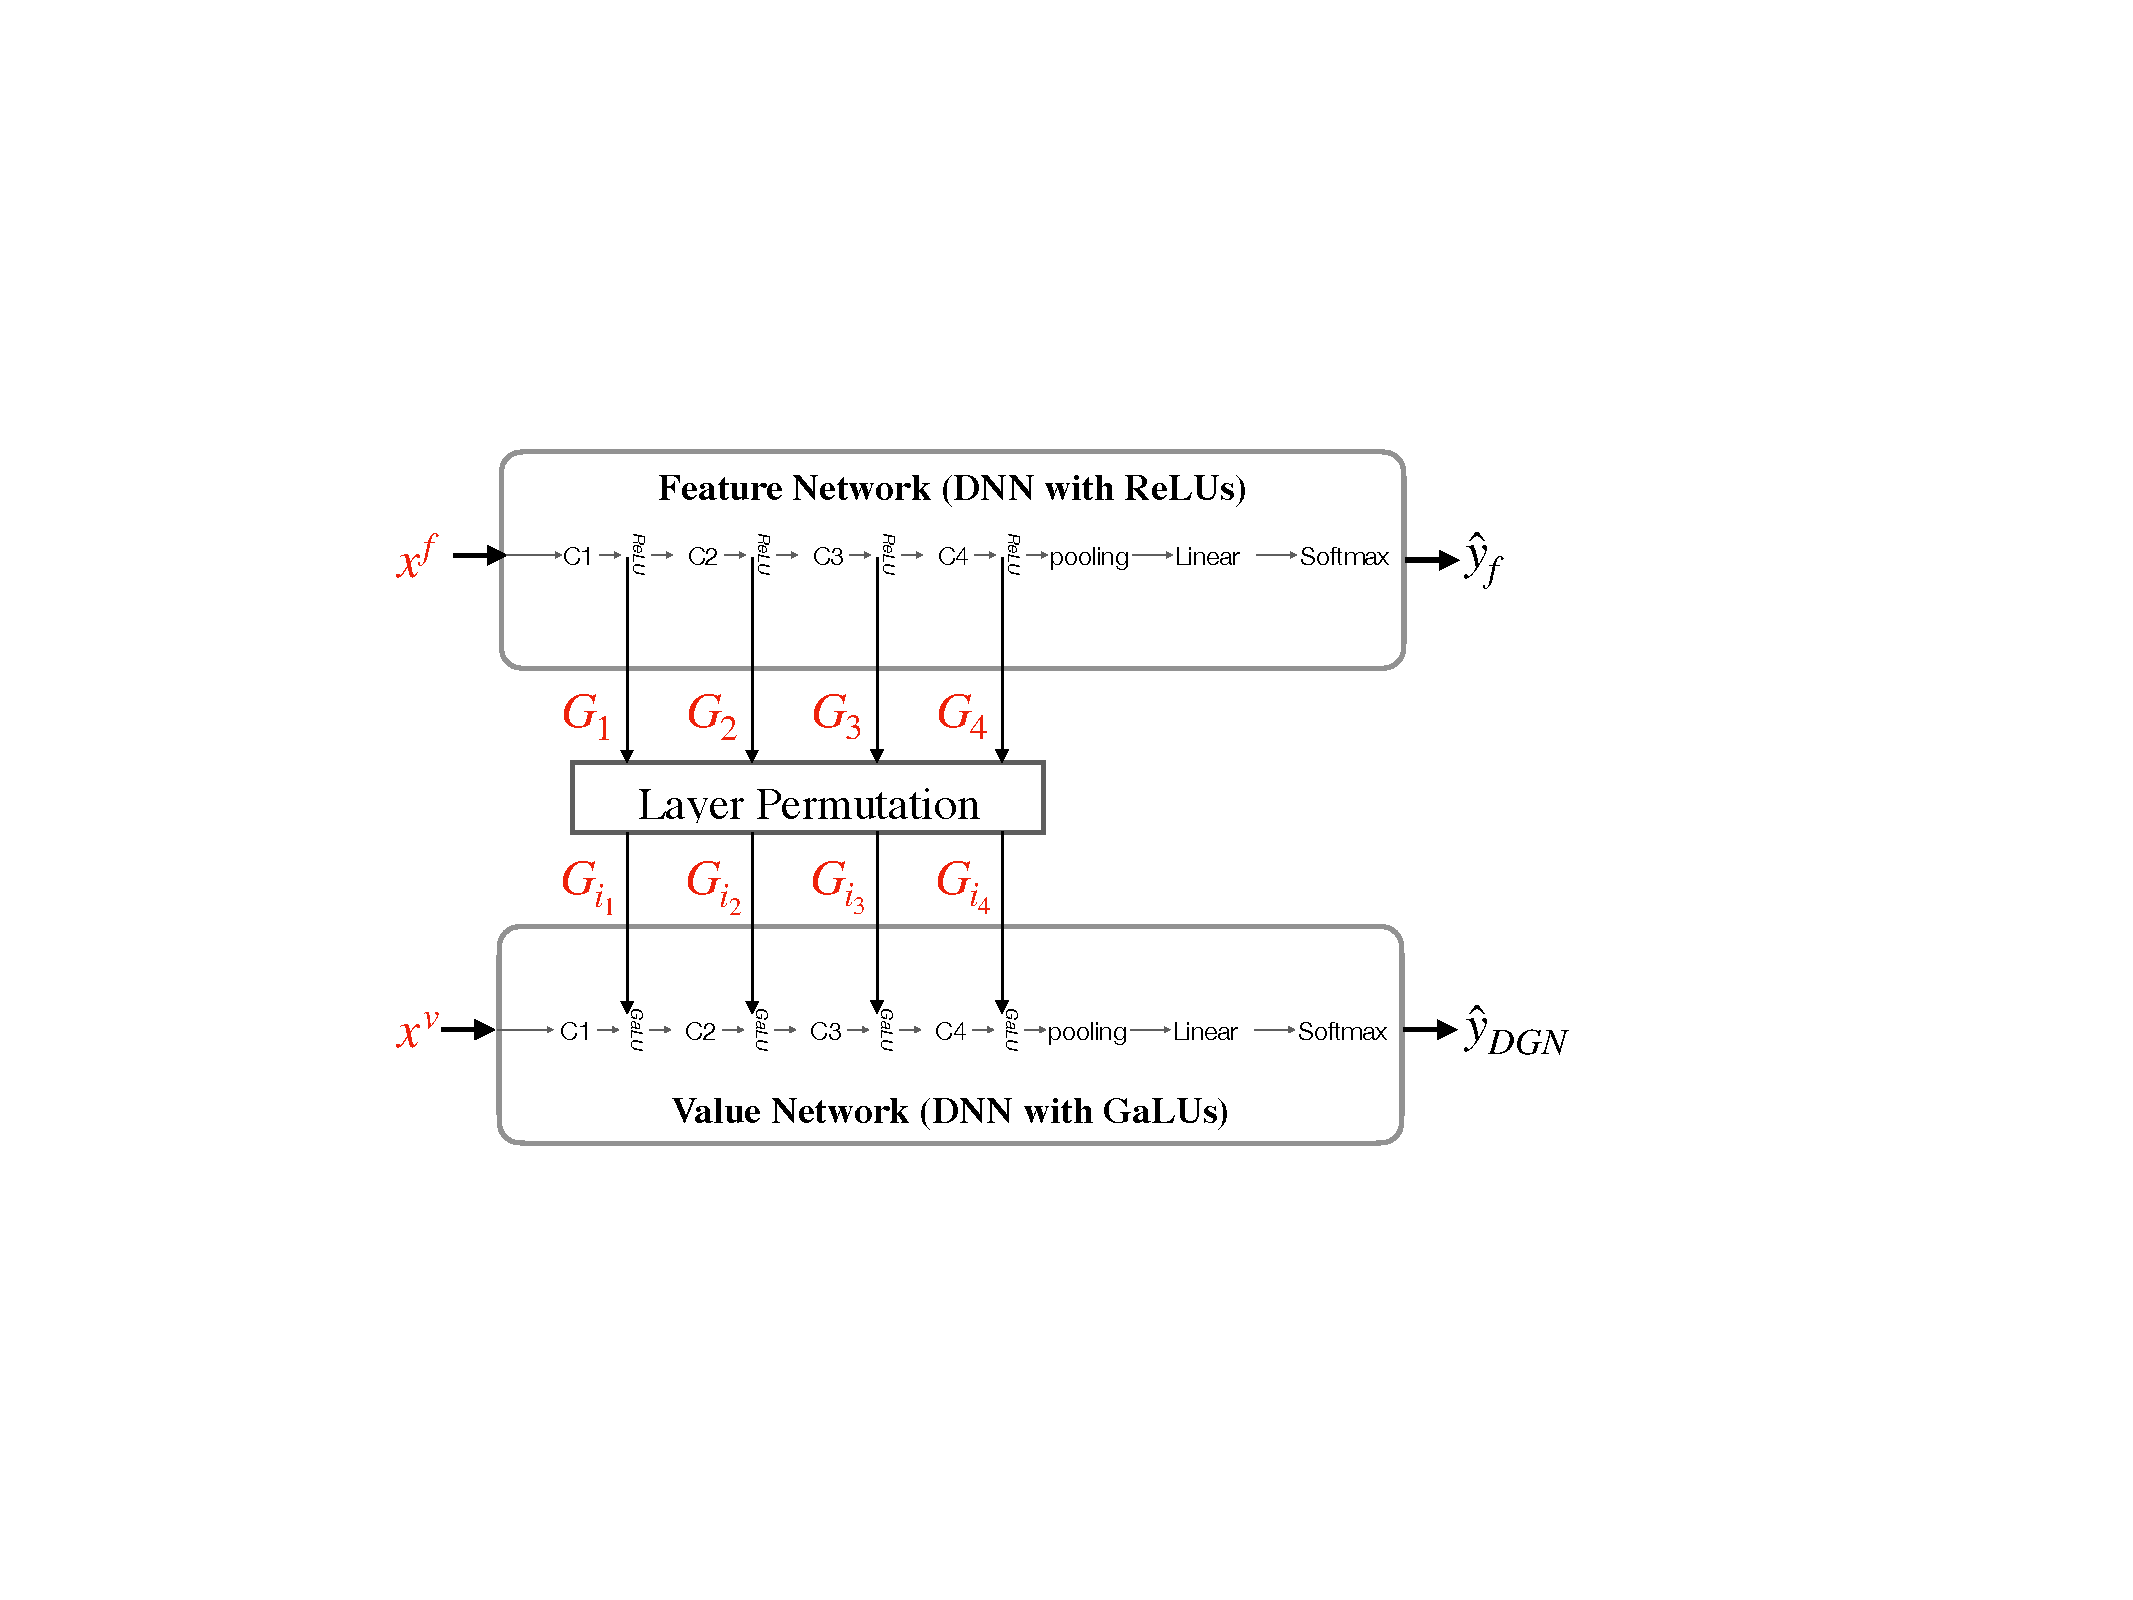
\includegraphics[scale=0.3]{figs/exp-new.pdf}
}
\end{minipage}
\caption{The prior setup in [\citenum{npk}] is shown in the left and the setup in this paper is shown in the right. Here $C1,\ldots,C4$ are convolutional layers with $128$ output filters, kernel size $3\times 3$ and stride $1\times 1$.}
\label{fig:dgn-prior-new}
\end{figure}

\textbf{This Paper (4 Regimes, 48 Models Per Regime ).} The improvisations are marked in {\color{red}{red}}.  In the current setup, {\bf{$G_{i_1},\ldots,G_{i_4}$ is a permutation of the $G_1,\ldots,G_4$}}, this gives $24$ models. In the prior setup both value and feature networks have the same input $x\in\R^{\din}$. In the current setup, we have two separate inputs, $x^{\text{f}}\in\R^{\din}$ for the feature network and $x^{\text{v}}\in\R^{\din}$ for the value network. We set $x^{\text{f}}=x$ always, however, for $x^{\text{v}}$ there are \textbf{two modes} namely (i) \textbf{standard}: we set $x^{\text{v}}=x$ ,(ii) \textbf{constant}: we set $x^{\text{v}}=\mathbf{1}\in\R^{\din}$ (a tensor of all $1$'s). While the setup on the left is only one model, the setup on the right has $\mathbf{48=24\times 2}$ \textbf{different models}, where $24=\texttt{factorial}(4)$ is due to the gate permutations and $2$ is due to the two different ways of setting $x^{\text{v}}$.






\begin{tabular}{|p{1.75cm}|c|c|c|c|c|}\hline
& FR-II &FR-DI & DL& FL& ReLU\\\hline
\centering{FC (MNIST)} &$94.1\%$  &$94.1\%$  &$98.1\%$ &$98.6\%$ &$98.5\%$\\\hline
\centering{CNN (CIFAR-10)}&$67.5\%$ &$67.6\%$   &$77.6\%$ &$79.4\%$ &$80.4\%$\\\hline
\end{tabular}


\textbf{Discussion.}

\indent\quad $1.$ \textbf{Decoupling gates and weights does not hurt.} There is no performance difference between FR-II and FR-DI.  Further, decoupled learning of gates (DL) performs significantly better than fixed random gates (FR), and the gap between standard DNN with ReLU and DL is less than $3\%$. This marginal performance loss seems to be worthy trade off for fundamental insights of \Cref{th:main} under the decoupling assumption.

\indent\quad $2.$ \textbf{Features are in the gates.} The fixed learnt regime (FL) shows that using the gates of a pre-trained ReLU network, performance can be recovered by training the NPV. Also, by interpreting the input dependent component of a model to be the features and the input independent component to be the weights, it makes sense to look at the gates/NPFs as the hidden features and NPV as the weights.% (which can be re-trained).

\indent\quad $3.$ \textbf{Random gates perform well.} FR-II does perform well in all the experiments (note that for a $10$-class problem, a random classifier would achieve only $10\%$ test accuracy). Given the observation that the gates are the true features, and the fact that is there no learning in the gates in the fixed regime, and the performance of fixed random gates can be purely attributed to the in-built structure.

\indent\quad $4.$ \textbf{Gate Learning explain finite vs infinite width.} We group the models into three sets where $S_1=\{$ ReLU, FL , DL$\}$, $S_2=\{$ FR$\}$ and $S_3=\{$ CNTK $\}$, and explain the difference in performance due to gate learning.
 $S_2$ and $S_3$ have no gate learning. However,  $S_3$ due to its infinite width has better averaging resulting in a well formed kernel and hence performs better than $S_2$ which is a finite width. Thus, the difference between $S_2$ and $S_3$ can be attributed to finite versus infinite width. Both $S_1$ and $S_2$ are finite width, and hence, conventional feature learning happens in both $S_1$ and $S_2$, but, $S_1$ with gate learning is better ($77.5\%$ or above in CIFAR-10) than $S_2$ ($67\%$ in CIFAR-10) with no gate learning. Thus neither finite width, nor the conventional feature learning explain the difference between $S_1$ and $S_2$. Thus, `gate learning' discriminates the regimes $S_1, S_2$ and $S_3$ better than the conventional feature learning view.

\indent\quad $5.$ \textbf{Robustness to layer permutation:} The performance (in all the $4$ regimes) is also robust to permutation of layers. Recall that the NPK expression in \Cref{th:main} is dependent on gating information in the form of $\ip{G_l(x),G_l(x')}$. So robustness to layer permutations is because, even if we permute the layers in the value network, whether or not any given gate triggers for both inputs $x$ and $x'$ remains invariant to this permutation. 

\indent\quad $6.$ \textbf{Robustness to constant input:} The performance (in all the $4$ regimes) is  robust to `all-ones' inputs. Note that in the `all-ones' case, the input information affects the models only via the gates. Here, all the entries of the input Gram matrix are identical, and the NPK depends only the correlation between the gates $\ip{G_l(x),G_l(x')}$.

\indent\quad $7.$ \textbf{Are Features Learnt Hierarchically? Yes and No.}

\begin{figure}[h]
\begin{minipage}{0.3\columnwidth}
\resizebox{\columnwidth}{!}{
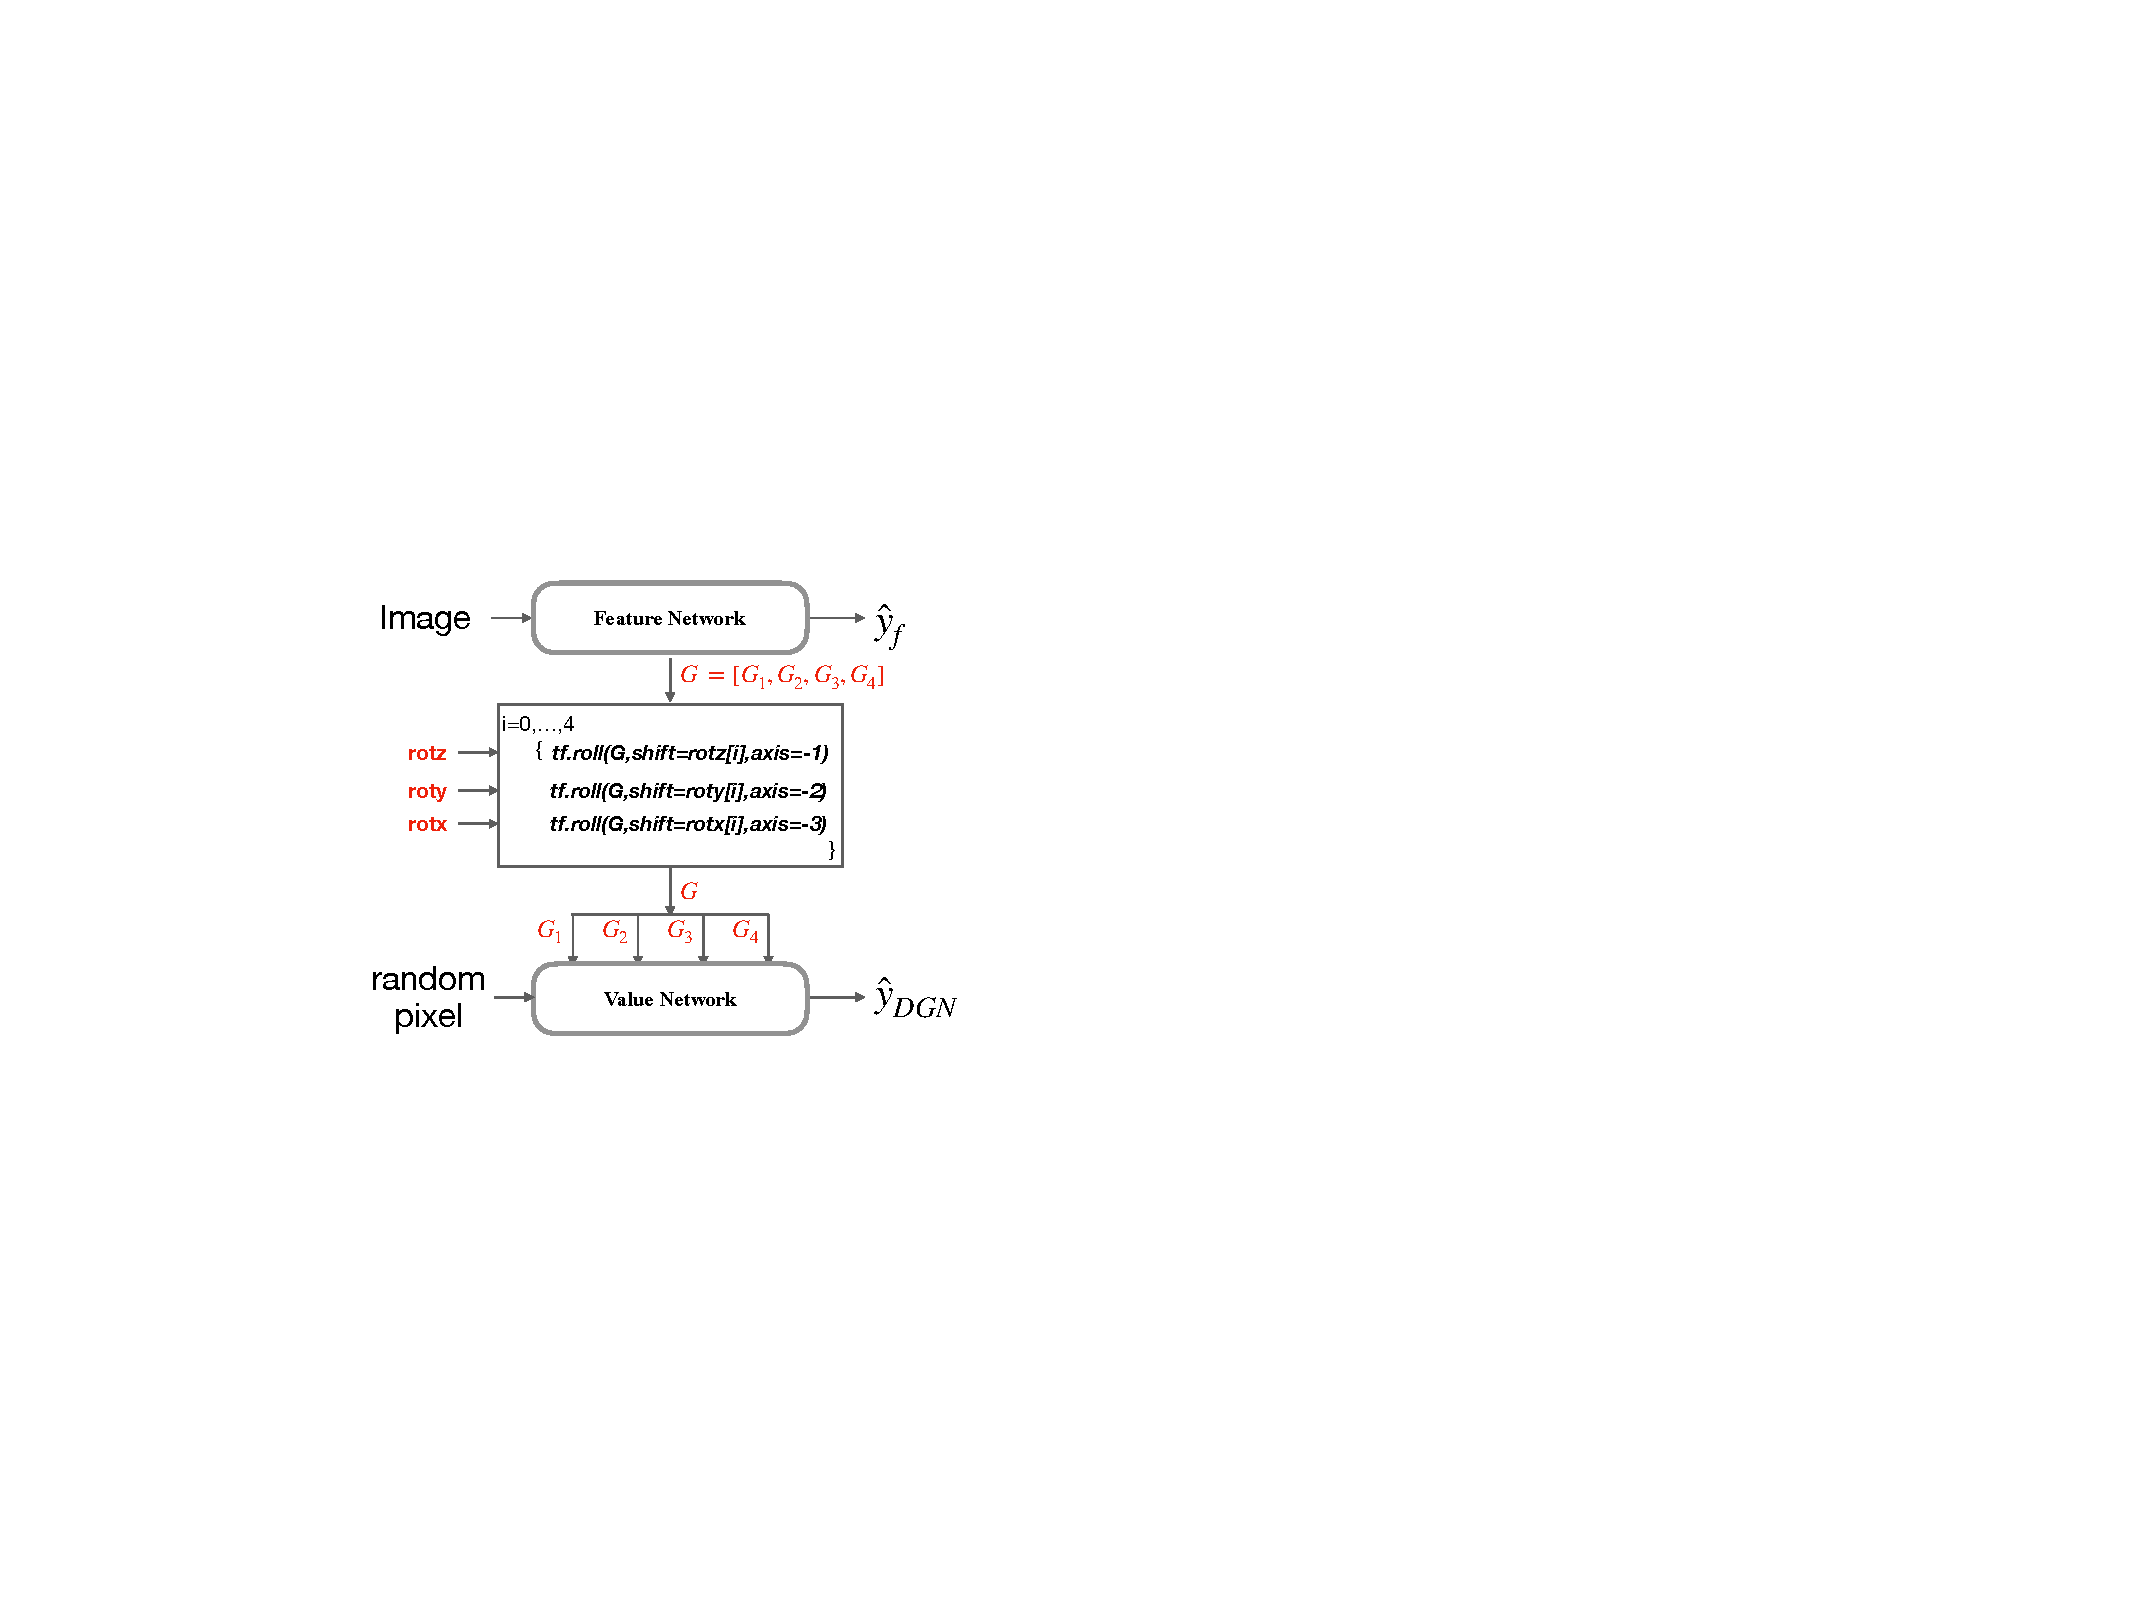
\includegraphics[scale=0.25]{figs/arbitrary_shift.pdf}
}
\end{minipage}
\begin{minipage}{0.68\columnwidth}
\resizebox{\columnwidth}{!}{
\begin{tabular}{cccccccccc}
&\Huge{Input}& \Huge{Layer 1, Filter 1}& \Huge{Layer 1, Filter 2}& \Huge{Layer 2, Filter 1}& \Huge{Layer 2, Filter 2}& \Huge{Layer 3, Filter 1}& \Huge{Layer 3, Filter 2}& \Huge{Layer 4, Filter 1}& \Huge{Layer 4, Filter 2}\\
\Huge{Feature Network}&\includegraphics{visual-iclr/images/horse.png}&
\includegraphics{images_neurips_2021/feature_network/layer_1_0.png}&
\includegraphics{images_neurips_2021/feature_network/layer_1_1.png}&
\includegraphics{images_neurips_2021/feature_network/layer_2_0.png}&
\includegraphics{images_neurips_2021/feature_network/layer_2_1.png}&
\includegraphics{images_neurips_2021/feature_network/layer_3_0.png}&
\includegraphics{images_neurips_2021/feature_network/layer_3_1.png}&
\includegraphics{images_neurips_2021/feature_network/layer_4_0.png}&
\includegraphics{images_neurips_2021/feature_network/layer_4_1.png}\\
\Huge{Value Network}&\includegraphics{images_neurips_2021/allones.png}&
\includegraphics{images_neurips_2021/value_network//layer_1_0.png}&
\includegraphics{images_neurips_2021/value_network//layer_1_1.png}&
\includegraphics{images_neurips_2021/value_network//layer_2_0.png}&
\includegraphics{images_neurips_2021/value_network//layer_2_1.png}&
\includegraphics{images_neurips_2021/value_network//layer_3_0.png}&
\includegraphics{images_neurips_2021/value_network//layer_3_1.png}&
\includegraphics{images_neurips_2021/value_network//layer_4_0.png}&
\includegraphics{images_neurips_2021/value_network//layer_4_1.png}
\end{tabular}
}

\end{minipage}
\caption{Top (Standard CNN): First image on the left is the input image and the next $8$ images are outputs of $2$ filters in each of the $4$ layers. Bottom (DGN with gates of the top model applied in reverse order): First image on the left is the input to the value network and the next $8$ images are outputs of $2$ filters in each of the $4$ layers. Both models achieve a test accuracy of about $80\%$.}
\label{fig:visual-permute}
\end{figure}



\subsection{Experiment 2: Upstream training with random labels and downstream with true labels}


\textbf{Q1 (open question).} {When trained with random labels upstream followed by true labels downstream, the test performance of DNNs with ReLUs degrades, Why?}

\textbf{Setup to answer Q1.} We hypothesise that the answer to the above question lies in the gates. To test our hypothesis, we train in two phases (i) Phase I: upstream training with label noise levels $\gamma=0, 25\%, 50\%, 75\%$ and (ii) Phase II: downstream training with true labels. We then measure the information stored in the gates at the end of each of the two phases. To this end, we consider the DGN setup in \Cref{fig:dgn-prior-new} (left), and train the feature network (which is a DNN with ReLUs). In `Phase I: Upstream', we train the feature network for different values of label noise $\gamma=0, 25\%, 50\%, 75\%$, which gives us models $M1(\gamma)$ (see \Cref{fig:rand-label-setup}). In order to measure the information in the gates learnt at the end of `Phase I: Upstream', we keep these gates fixed and train the value network with true labels -- this gives us models $M2(\gamma)$ (see \Cref{fig:rand-label-setup}). Second is `Phase II: Downstream', wherein, we start with models $M1(\gamma)$, and perform downstream training with true labels to obtain models $M4(\gamma)$ ($\gamma=0$ is an exception; there is no downstream training because $M1(0)$ has been already trained with true labels in upstream).  In order to measure the information in the gates learnt at the end of `Phase II: Downstream', we keep these gates fixed and train the value network with true labels -- this gives us models $M5(\gamma)$ (see \Cref{fig:rand-label-setup}).

\begin{figure}[h]
\centering
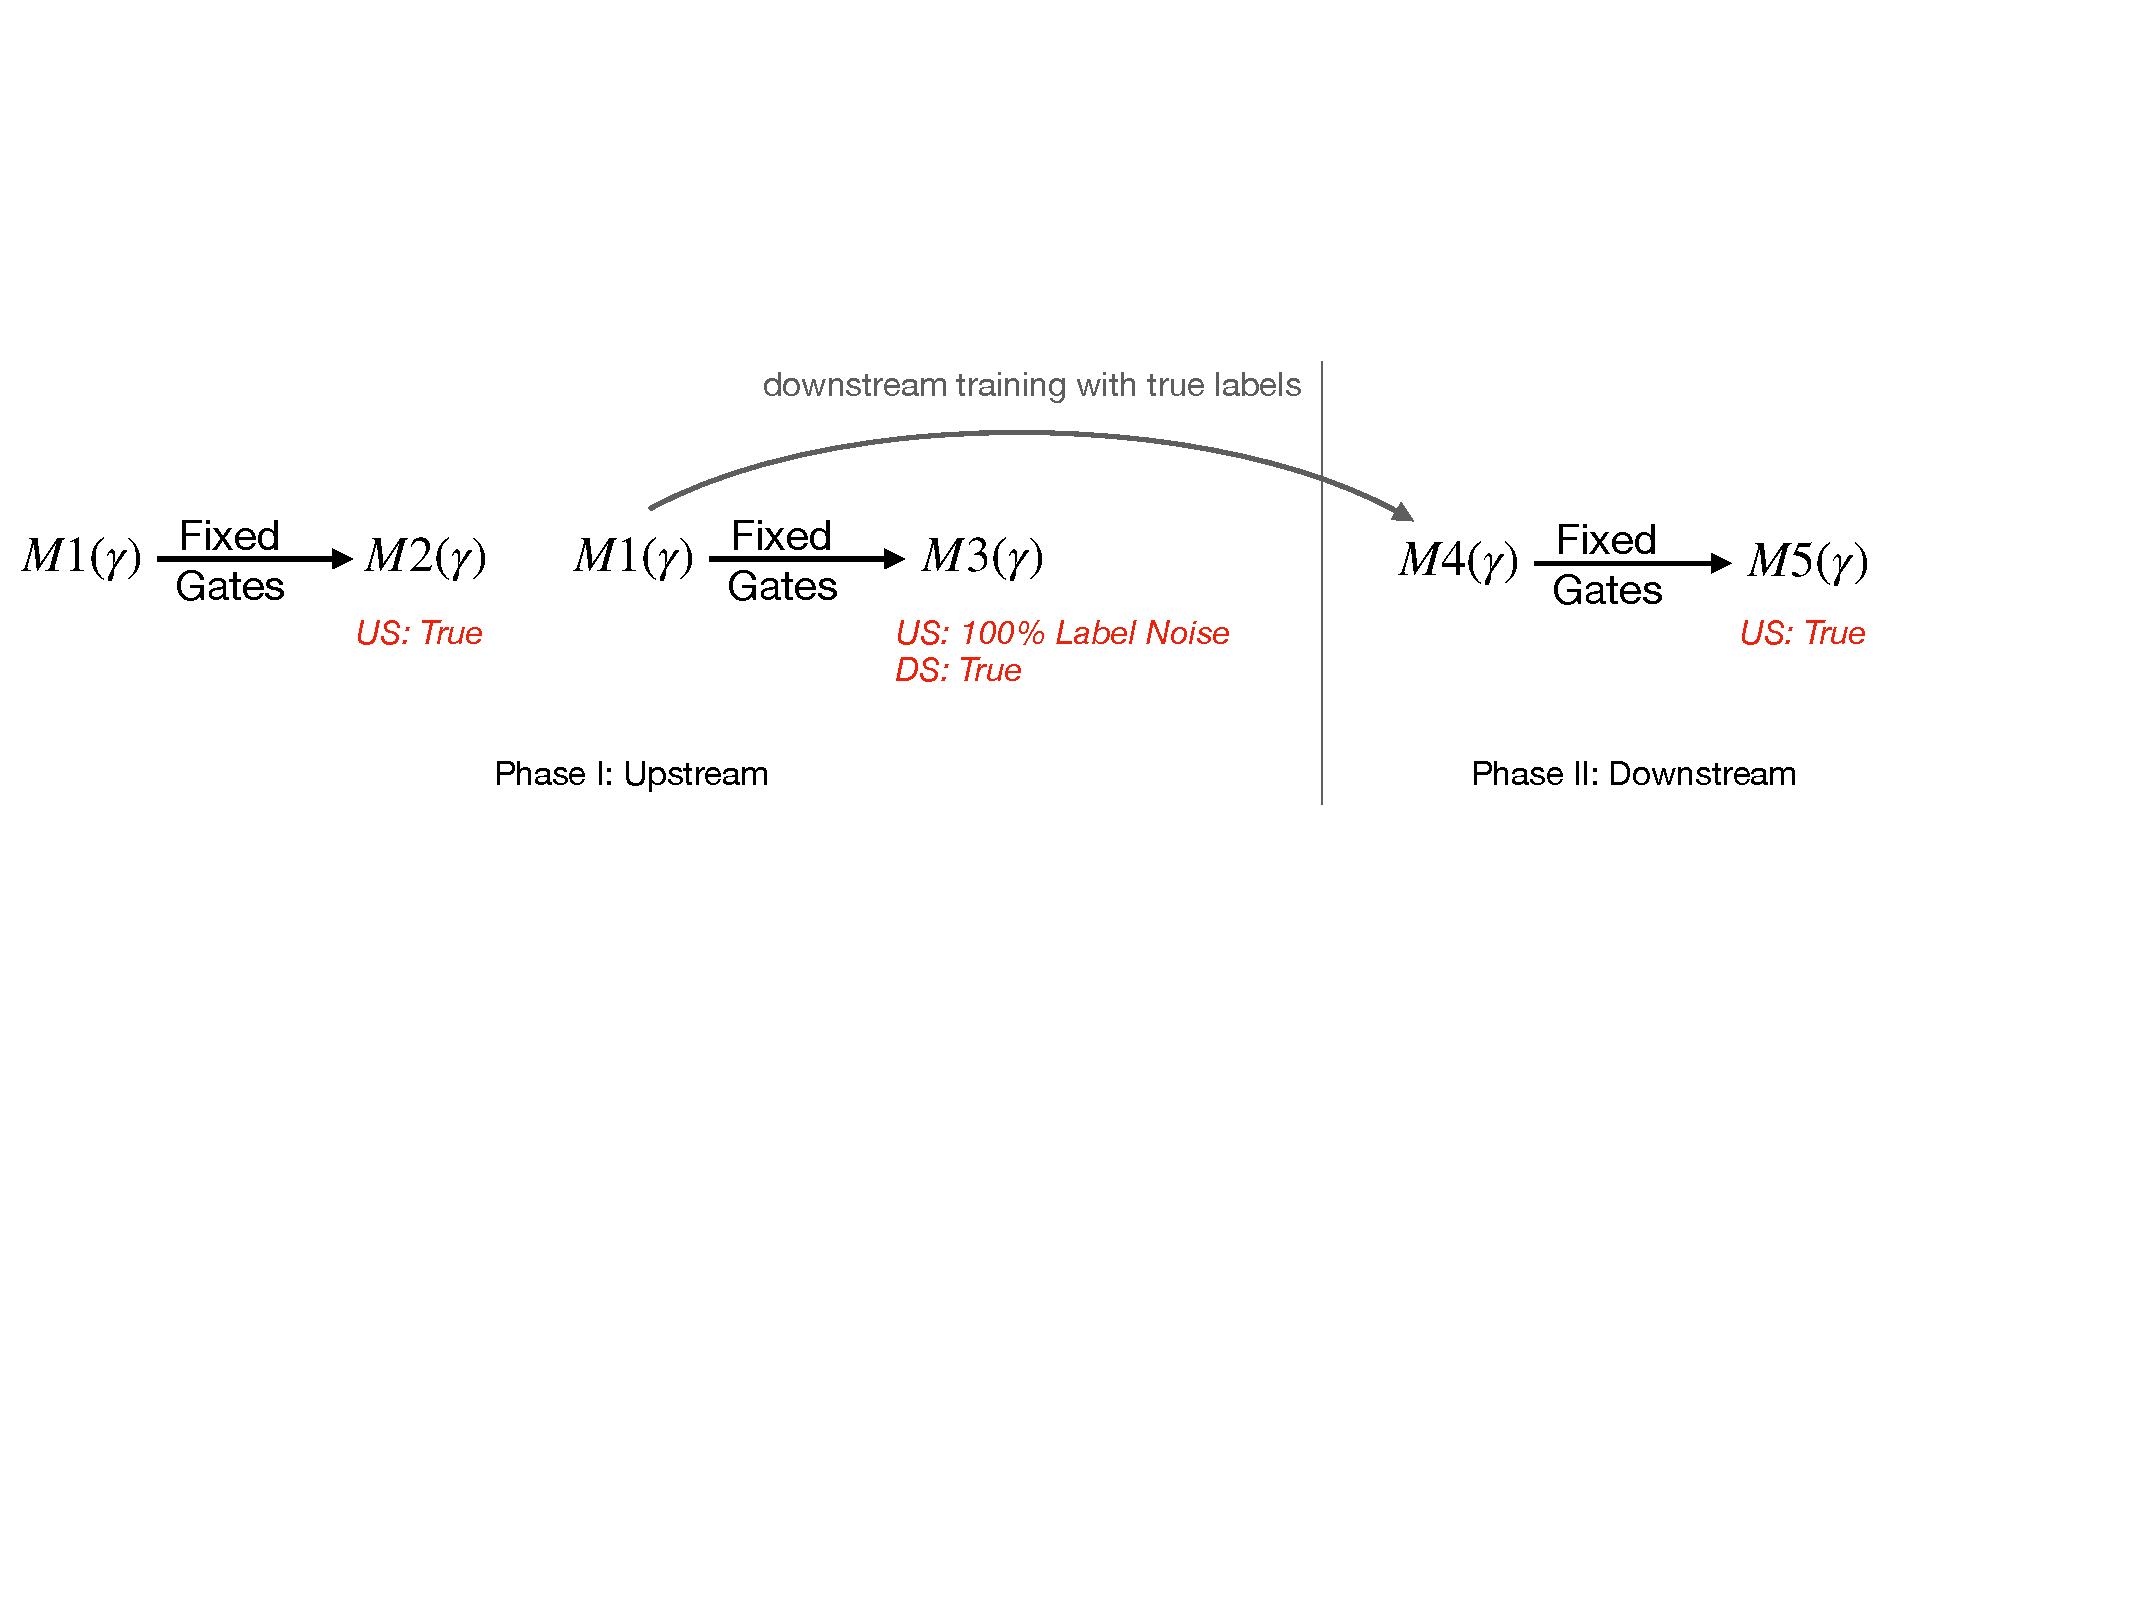
\includegraphics[scale=0.3]{figs/rand-label-big.pdf}
\caption{Shows various models trained in Experiment 2. Here, US and DS stand for upstream and down stream respectively. True for with true labels. Here models $M1$ and $M4$ are feature networks (DNNs with ReLUs), and $M2, M3$ and $M5$ are value networks which use the fixed gates from the feature networks. Models are parameterised by $(\gamma)$ which is the label noise level.}
\label{fig:rand-label-setup}
\end{figure}


\textbf{Q2 (new question).} {When trained with random labels upstream followed by true labels downstream, \emph{if the gates are fixed throughout and only the weights are trained}, does the test performance degrade?}

\textbf{Setup to answer Q2.} Here, we pick up the models trained at the end of `Phase I: Upstream', use them as feature networks and fix the gates. We then train the value network, first upstream with with $100\%$ random labels, and then downstream with $100\%$ true labels--this gives us models $M3(\gamma)$.

We now discuss the results of the experiments with random labels shown in \Cref{tb:rand-label} and \Cref{fig:rand-label}. 

\textbf{Answer to Q2.} \emph{When the gates are fixed test performance is robust to upstream training with random labels.} In  \Cref{tb:rand-label}, look at the performance of $M2(\gamma=0)$ and compare it performance of  $M4(\gamma), \gamma=25,50.75$. When the gates are fixed, the upstream training with even $100\%$ label noise does not hurt the test performance so much (less than $2\%$ for $\gamma=100$) in comparison to the cases when the gates are allowed to change (as it is the case of DNN with ReLUs), the test performance degrades (from $81.2$) to $76.9$ ( $ 4.3\%$ for $\gamma=25$), $73.6$ ( $7.6\%$ for $\gamma=50$) and  $68.1$ ($13.1\%$ for $\gamma=75$) for even less than $100\%$ label noise.



\begin{table}[h]
\begin{tabularx}{\columnwidth}{c *{6}{Y}}
\toprule

 & \multicolumn{4}{c}{Phase I: Upstream}  
 & \multicolumn{2}{c}{Phase II: Downstream}\\
\cmidrule(lr){2-5} \cmidrule(l){6-7}
&  \multicolumn{2}{c}{ReLU}  &\multicolumn{2}{c}{Fixed Gates} & ReLU & {Fixed Gates}\\
\cmidrule(lr){2-3} \cmidrule(lr){4-5}\cmidrule(lr){6-7}
$\gamma$& Best & End & True& US/DS & True & True\\\hline\arrayrulecolor{white}\midrule
0 &{\bf{81.2}}{\tiny $\pm$ 0.3} & 80.0{\tiny $\pm$ 0.4} &{\bf{80.3}}{\tiny $\pm$ 0.2} & {\bf{79.3}}{\tiny $\pm$ 0.4} &-&- \\\hline\hline
{25}&76.1{\tiny $\pm$ 0.6} & 63.1{\tiny $\pm$ 0.7}& 74.7{\tiny $\pm$ 0.5}& 72.3{\tiny $\pm$ 0.2}&76.9{\tiny $\pm$ 0.1}&76.9{\tiny $\pm$ 0.4}\\\hline\hline
{50}&70.9{\tiny $\pm$ 0.8} & 41.5{\tiny $\pm$ 1.1}& 69.9{\tiny $\pm$ 0.3} & 66.8{\tiny $\pm$ 0.1}&73.4{\tiny $\pm$ 0.3}&73.6{\tiny $\pm$ 0.4}\\\hline\hline
{75}&56.9{\tiny $\pm$ 0.4} & 23.4{\tiny $\pm$ 0.4}& 63.9{\tiny $\pm$ 0.4} &60.0{\tiny $\pm$ 0.3}&68.1{\tiny $\pm$ 0.4}&67.7{\tiny $\pm$ 0.6}\\\hline
\arrayrulecolor{black}\bottomrule
Models & \multicolumn{2}{c}{M1($\gamma$)} & M2($\gamma$) & M3($\gamma$)& M4($\gamma$) & M5($\gamma$)\\\bottomrule
\end{tabularx}
\caption{Shows the performance of the various models in Experiment 2.}
\label{tb:rand-label}
\end{table}


\textbf{Answer to Q1.} \emph{When training with random labels upstream, the test performance degrades because the gates get degraded.} This follows from the fact that the performance of the DNN with ReLUs at the end of `Phase II: Downstream', i.e., $M4$ and that of the value network with the fixed gates at end of `Phase II: Downstream', i.e., $M5$ are approximately equal (within $0.5\%$). 

\textbf{Gates are fairly robust to random labels.} Note that while training with random labels upstream, the test performance initially improves, reaches a peak and then degrades (see top row of \Cref{fig:rand-label}). The performance of the DNN with ReLUs at the end of `Phase I' is shown in the second column of \Cref{tb:rand-label}. However, the performance of the fixed gates at the end of `Phase I' shown in third column of \Cref{tb:rand-label} is much better and is more closer to the performance of the downstream model $M4$. This means, during upstream training with random labels, the performance degradation post the peak value mostly affects only the weights and not the gates.


\begin{figure}[h]
\begin{minipage}{0.99\columnwidth}
\resizebox{\columnwidth}{!}{
\begin{tabular}{ccc}
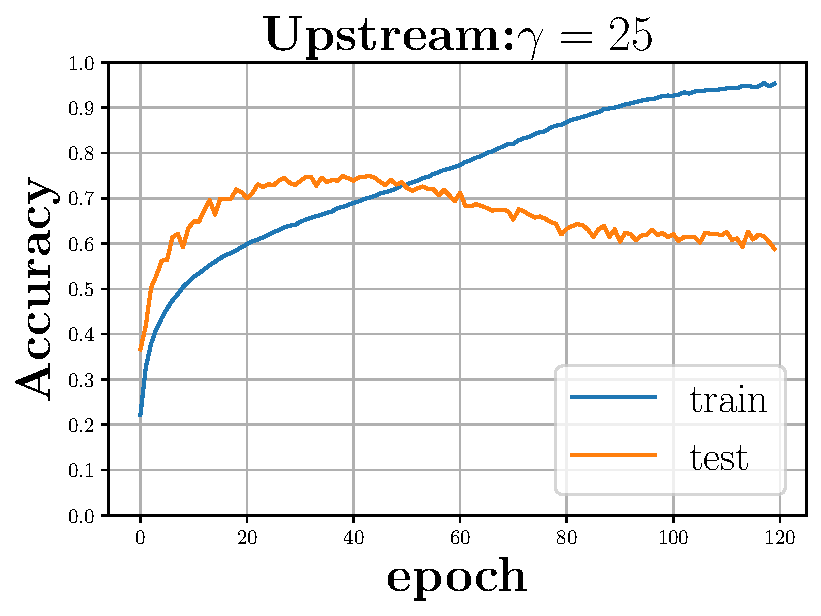
\includegraphics[scale=0.125]{figs/relu_25.pdf}&
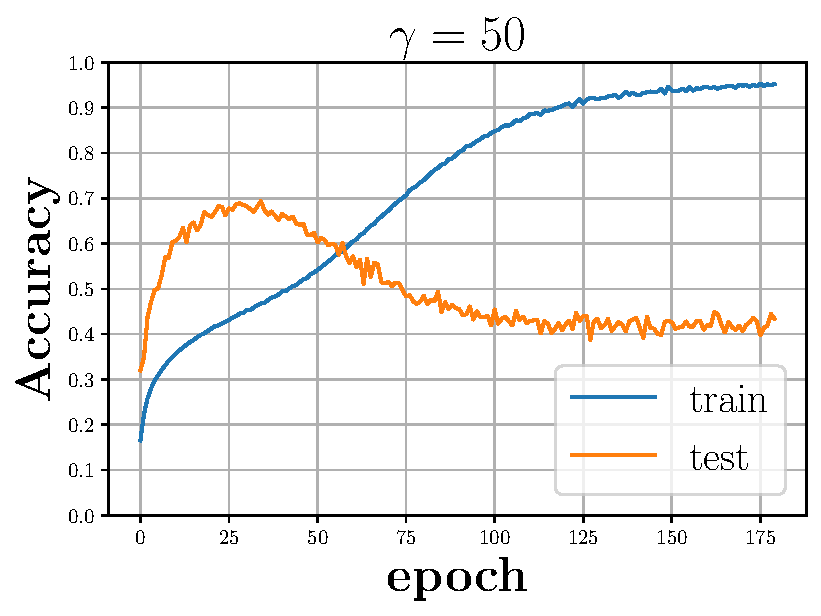
\includegraphics[scale=0.125]{figs/relu_50.pdf}&
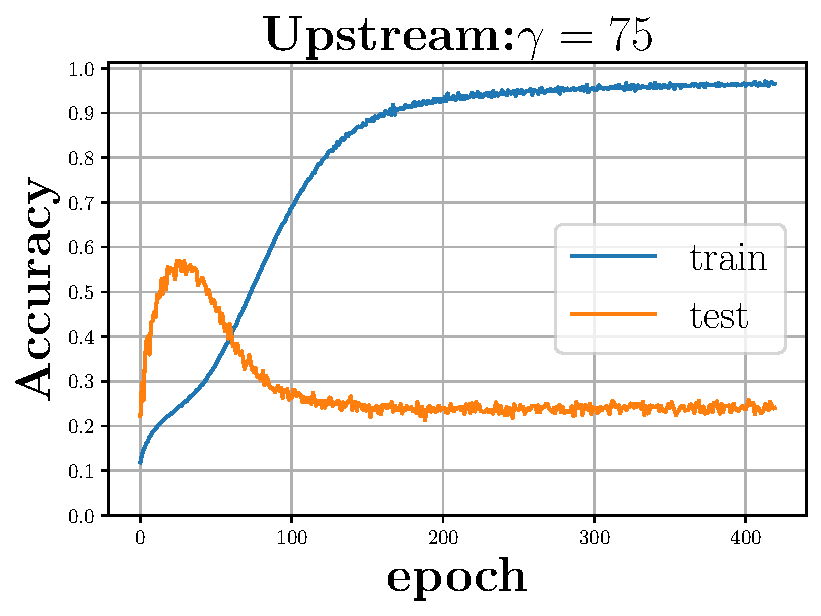
\includegraphics[scale=0.125]{figs/relu_75.pdf}
\\
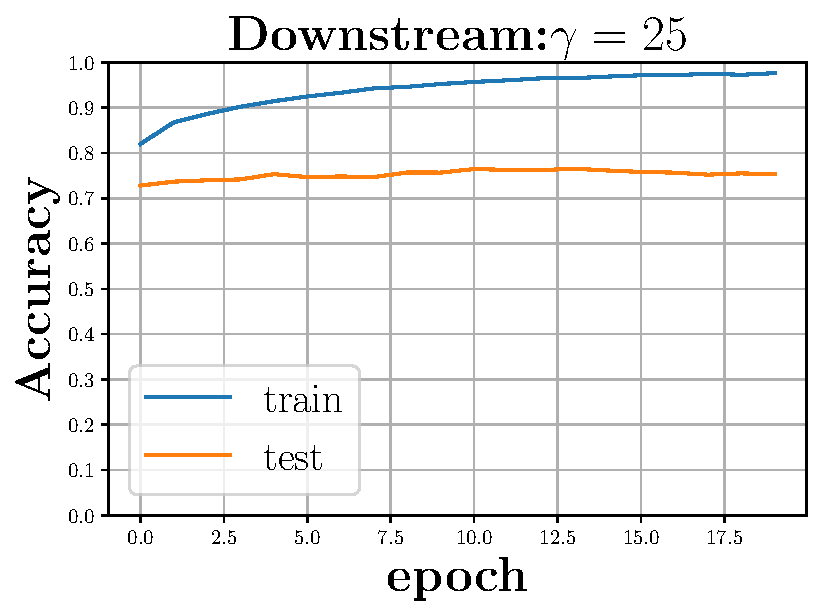
\includegraphics[scale=0.125]{figs/relu_25_good.pdf}&
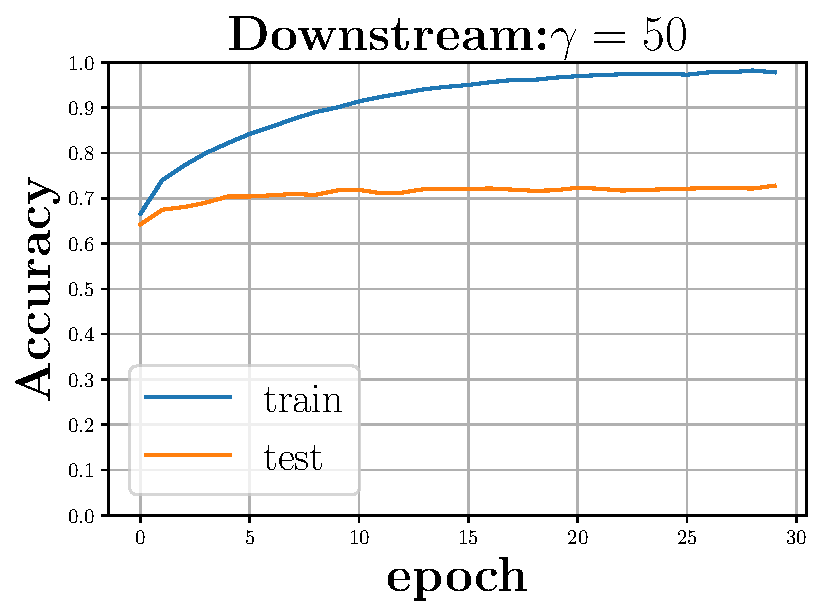
\includegraphics[scale=0.125]{figs/relu_50_good.pdf}&
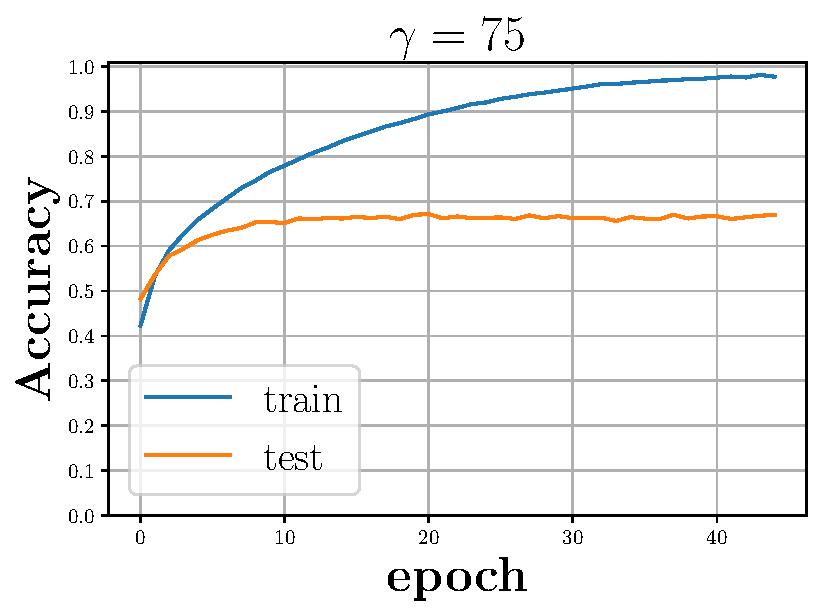
\includegraphics[scale=0.125]{figs/relu_75_good.pdf}\\
\end{tabular}
}
\end{minipage}
\caption{Shows the upstream training with random labels followed downstream training with true labels. The first epochs of bottom plots is same as the epoch follows the last epoch in the top plots.}
\label{fig:rand-label}

\end{figure}


\begin{comment}
\begin{figure}[h]
%\begin{comment}
\begin{minipage}{0.4\columnwidth}
\resizebox{\columnwidth}{!}{
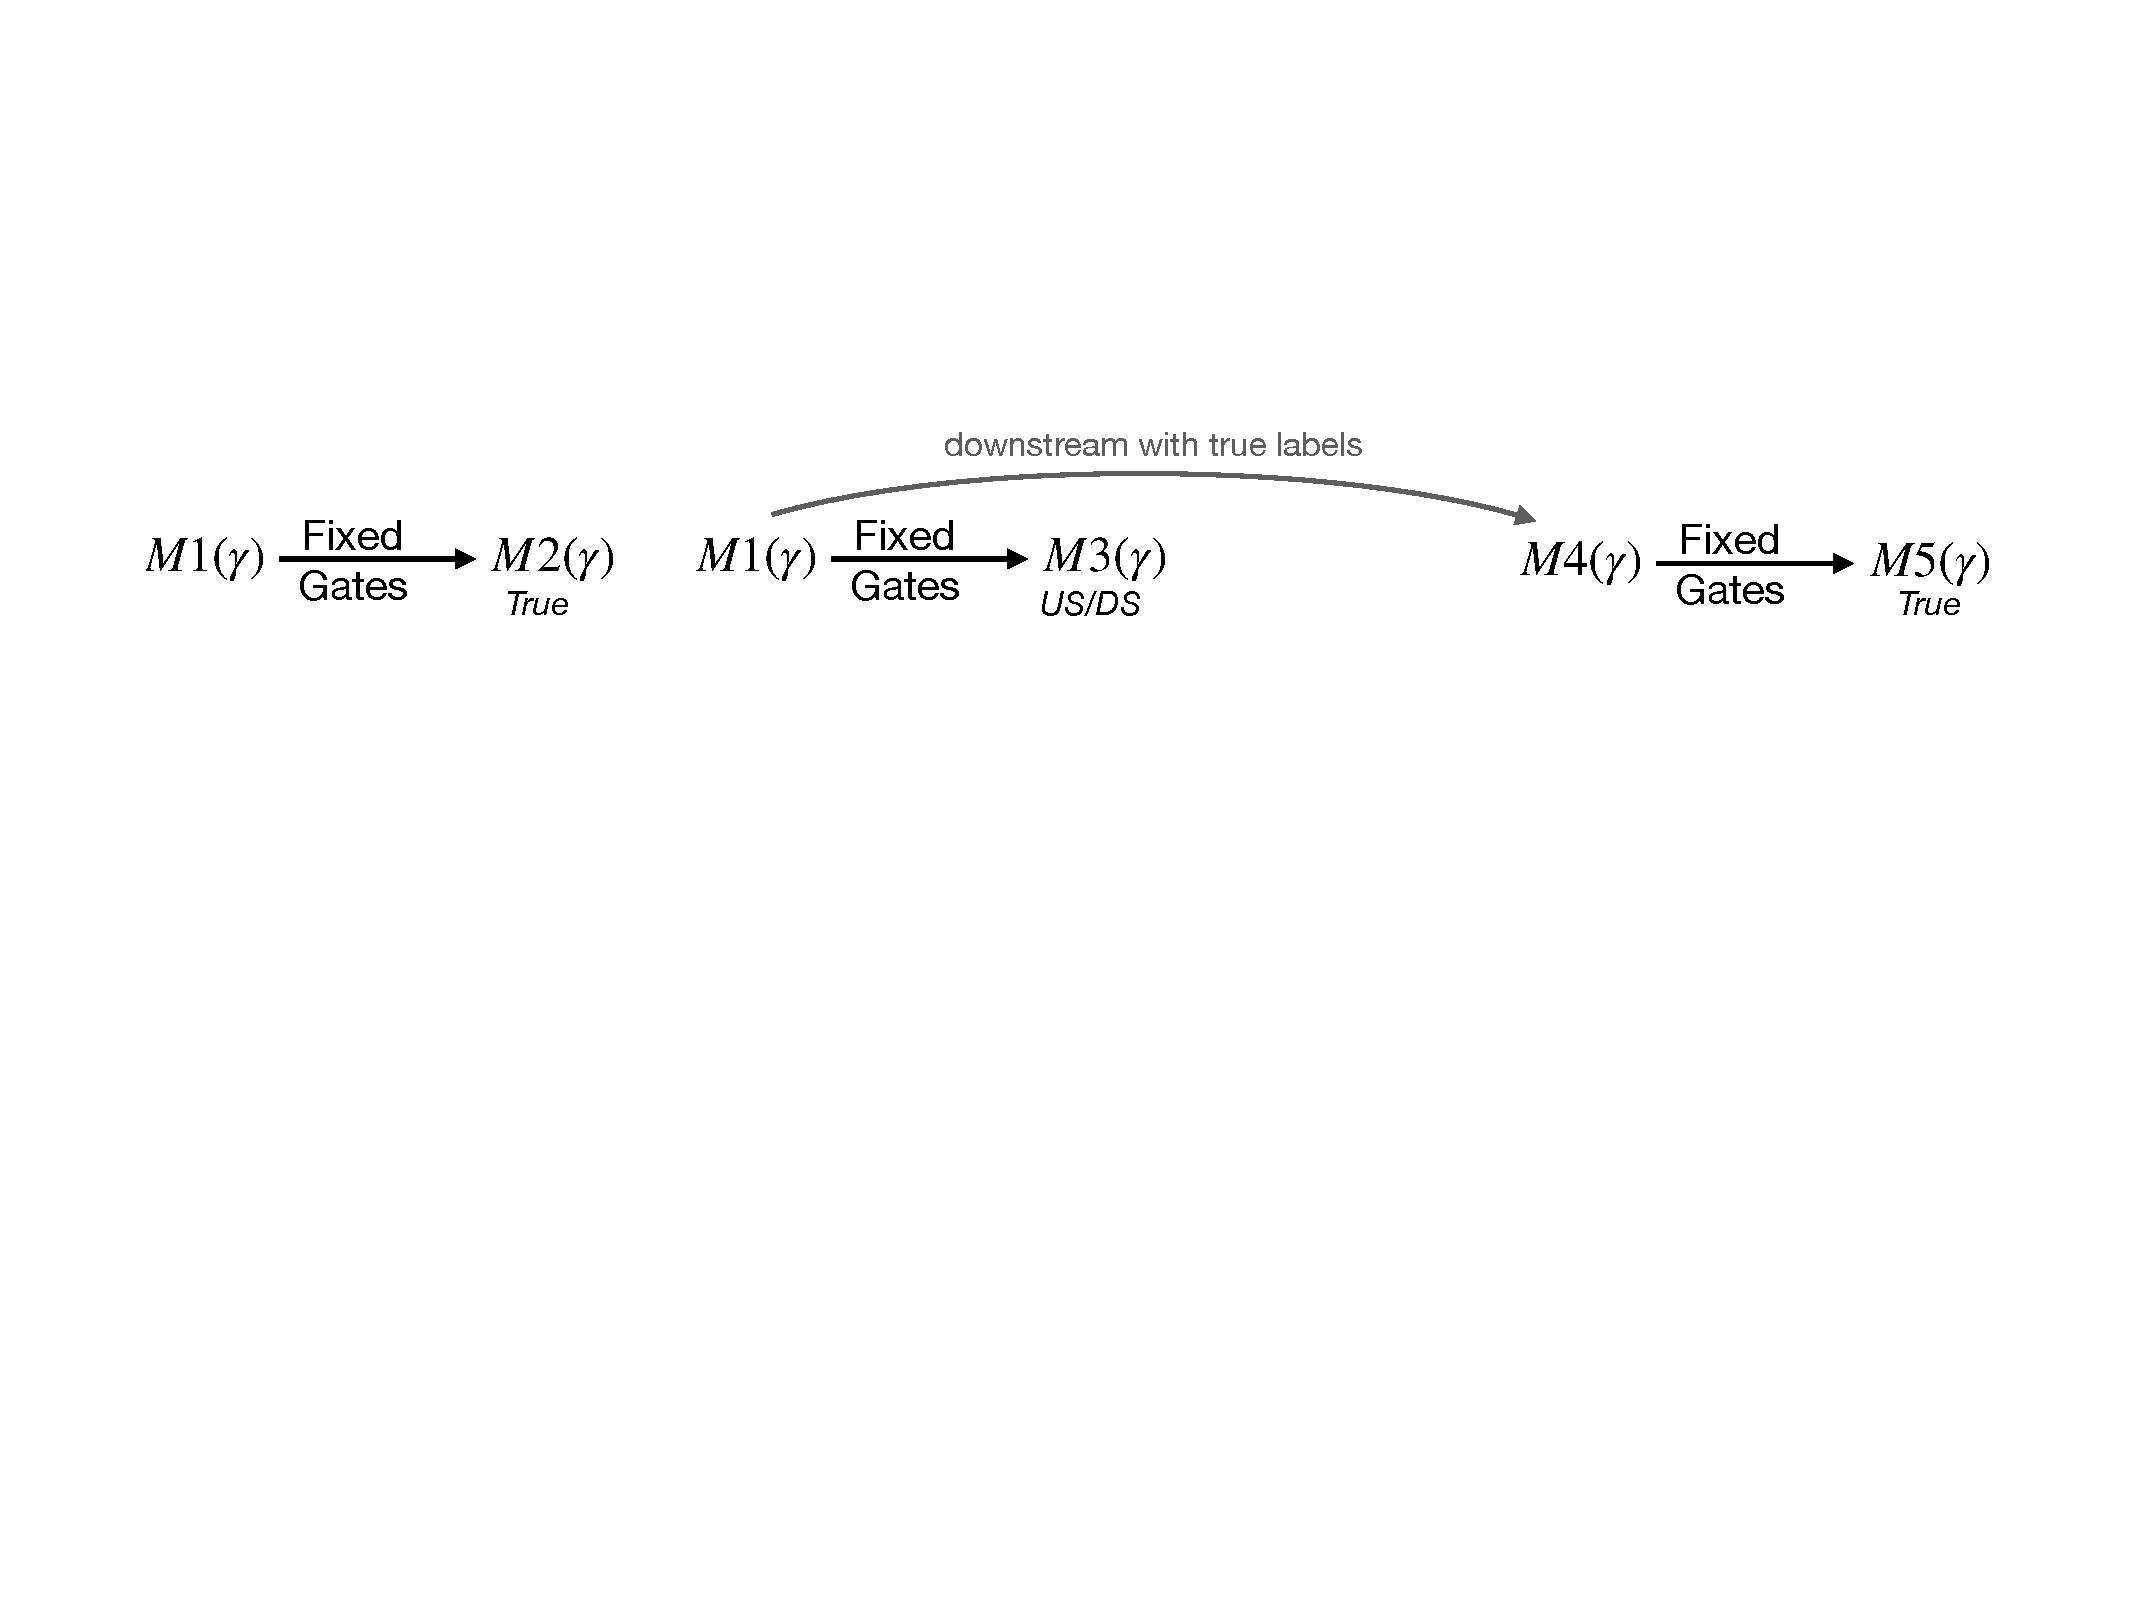
\includegraphics[scale=0.35]{figs/rand-label.pdf}
}
\end{minipage}
%\end{comment}
\begin{minipage}{0.99\columnwidth}
\resizebox{\columnwidth}{!}{
\begin{tabular}{cccccc}
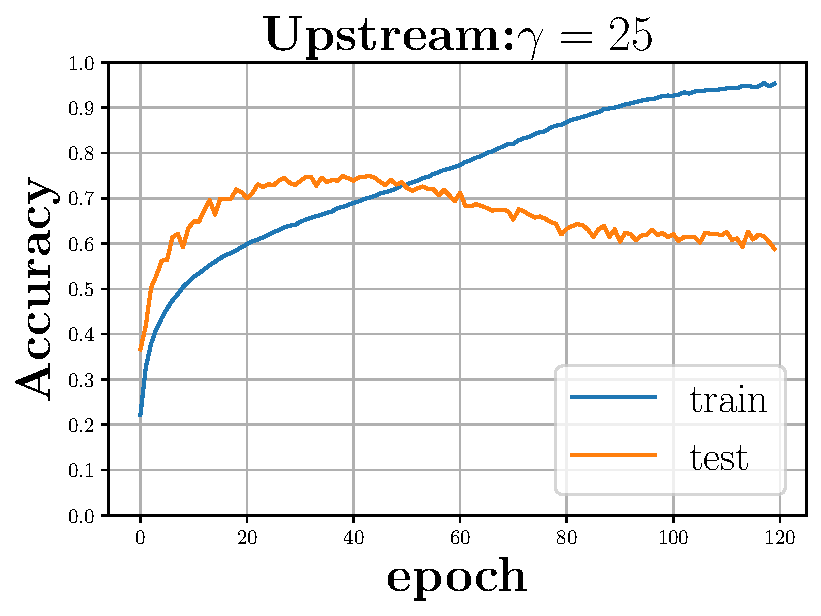
\includegraphics[scale=0.125]{figs/relu_25.pdf}&
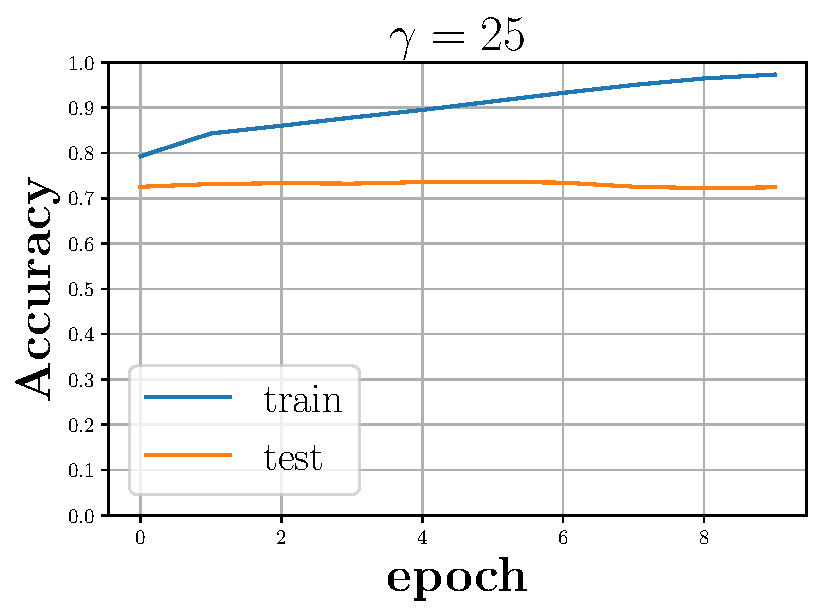
\includegraphics[scale=0.125]{figs/galu_25_good.pdf}&
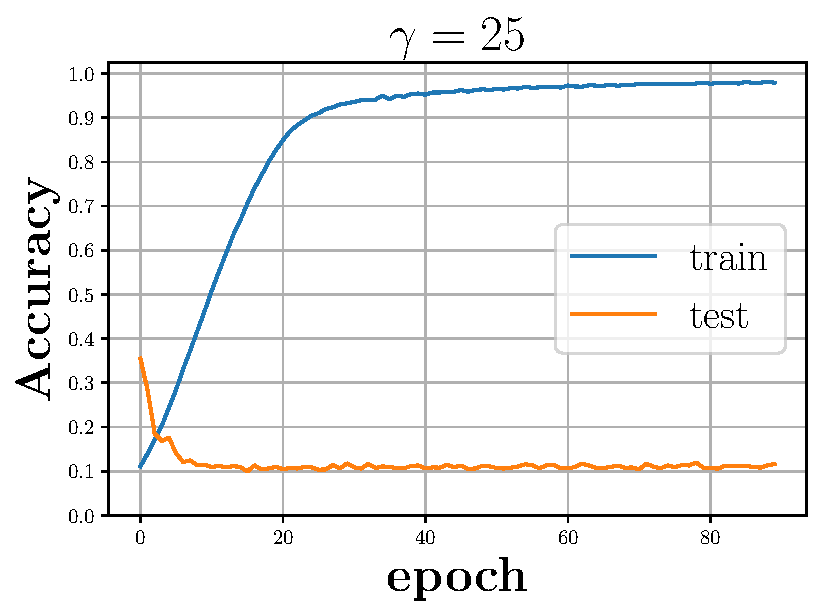
\includegraphics[scale=0.125]{figs/galu_25_bad.pdf}&
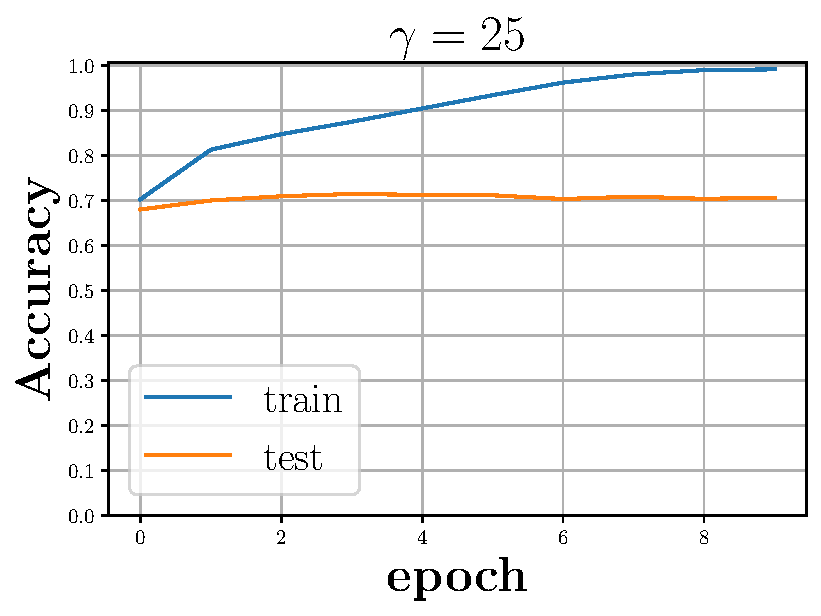
\includegraphics[scale=0.125]{figs/galu_25_bad_good.pdf}&
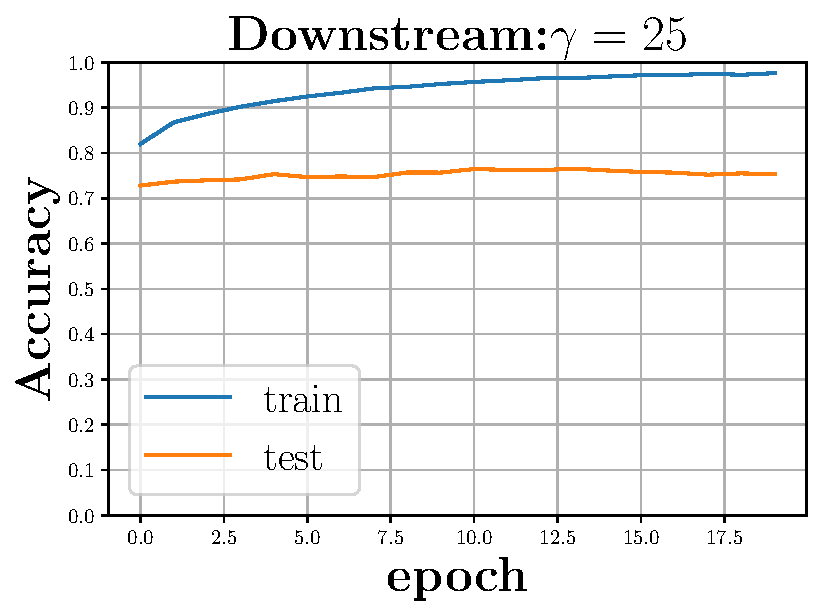
\includegraphics[scale=0.125]{figs/relu_25_good.pdf}&
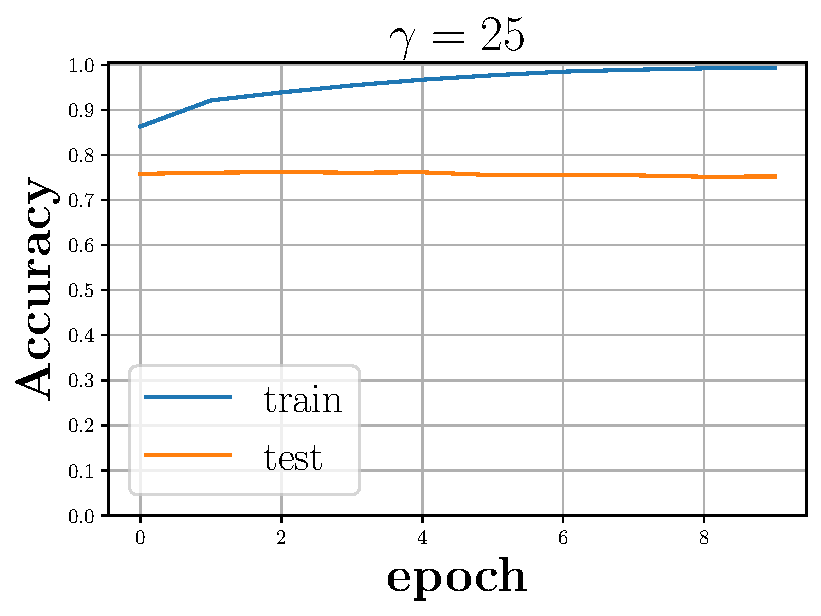
\includegraphics[scale=0.125]{figs/galu_25_recovered.pdf}
\\
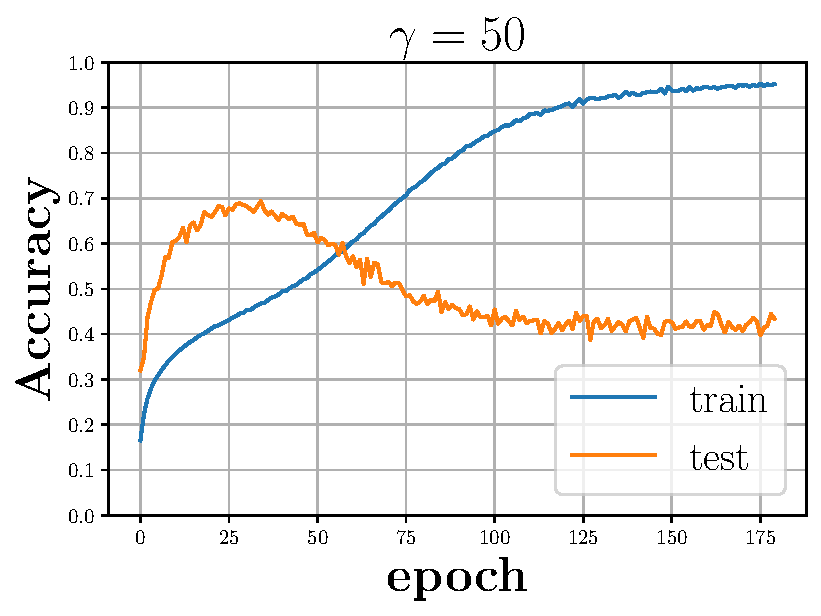
\includegraphics[scale=0.125]{figs/relu_50.pdf}&
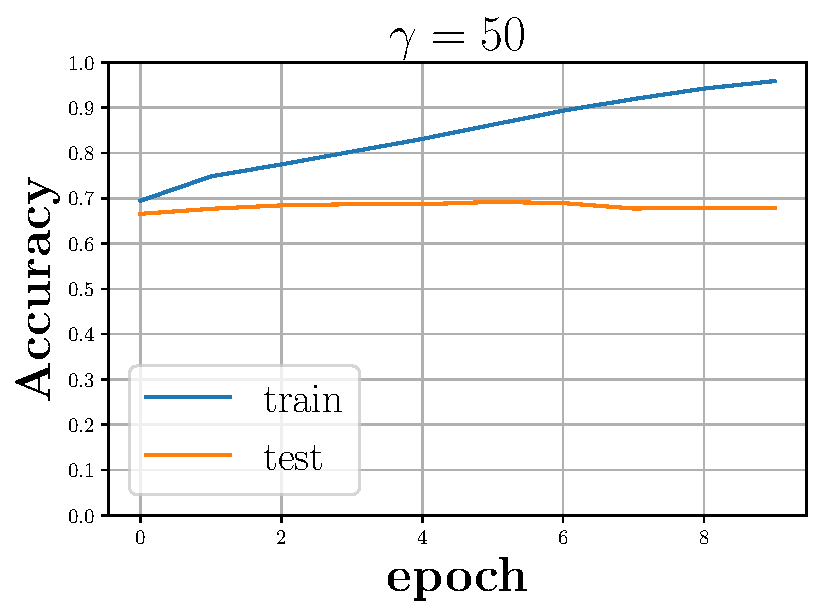
\includegraphics[scale=0.125]{figs/galu_50_good.pdf}&
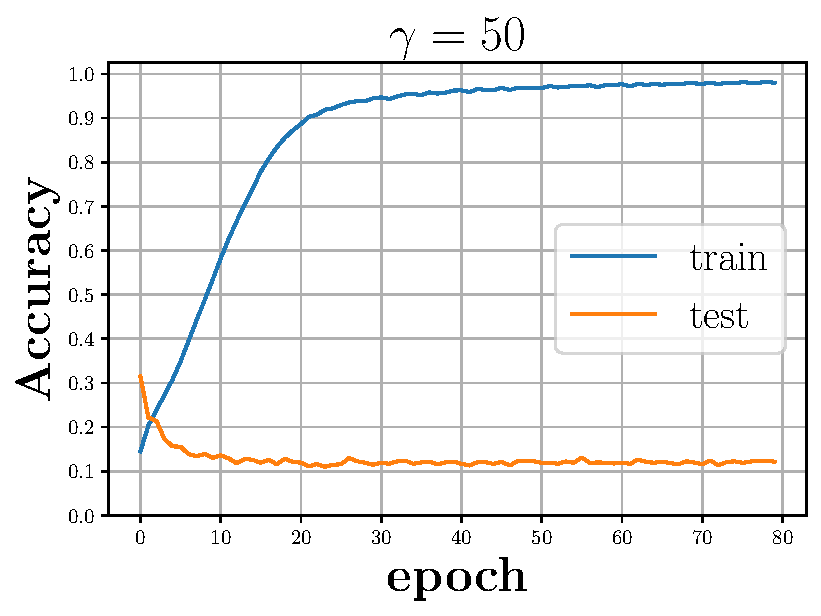
\includegraphics[scale=0.125]{figs/galu_50_bad.pdf}&
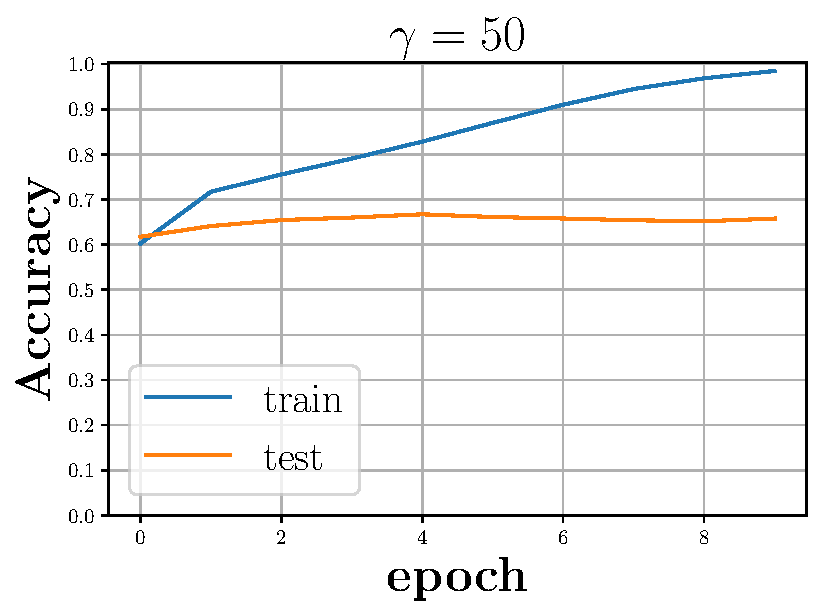
\includegraphics[scale=0.125]{figs/galu_50_bad_good.pdf}&
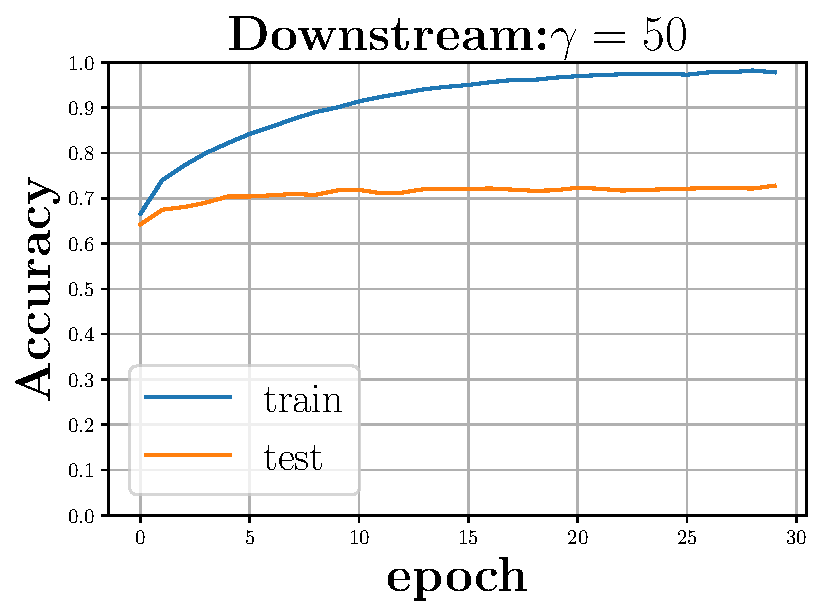
\includegraphics[scale=0.125]{figs/relu_50_good.pdf}&
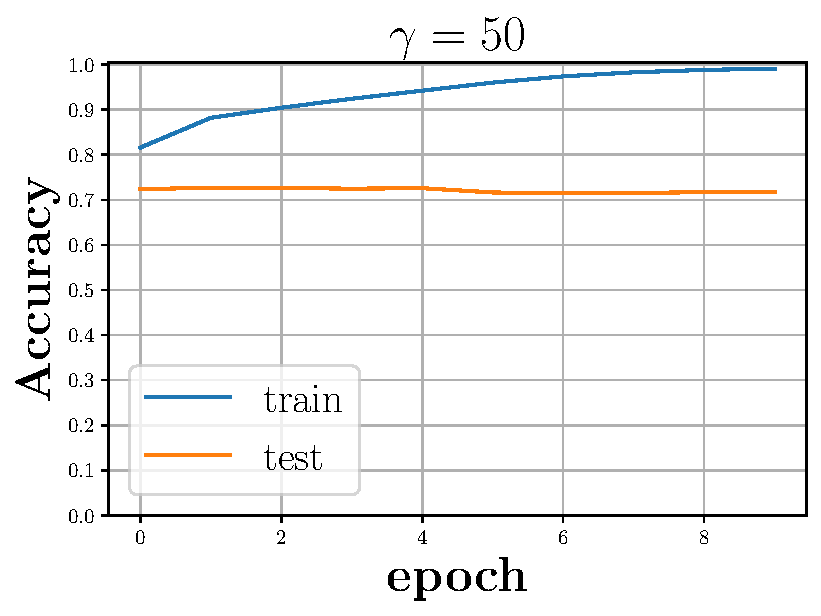
\includegraphics[scale=0.125]{figs/galu_50_recovered.pdf}
\\
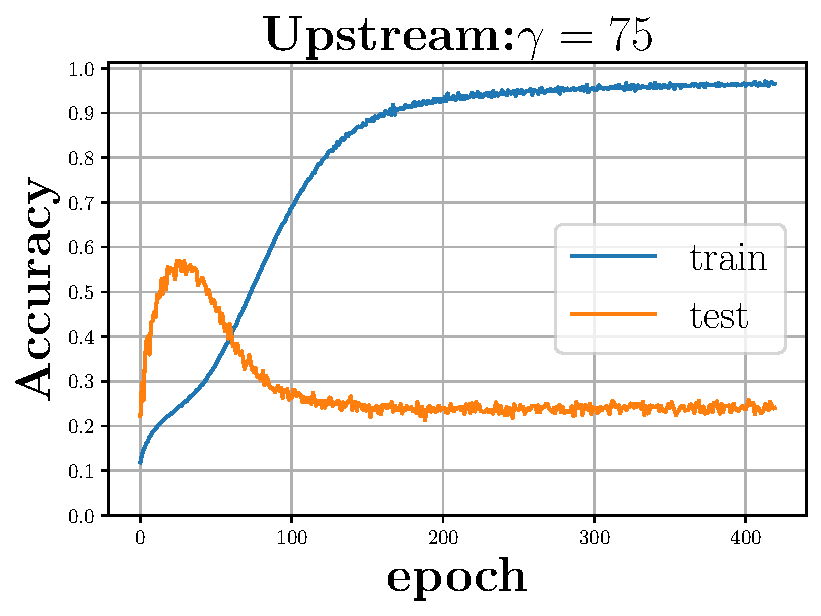
\includegraphics[scale=0.125]{figs/relu_75.pdf}&
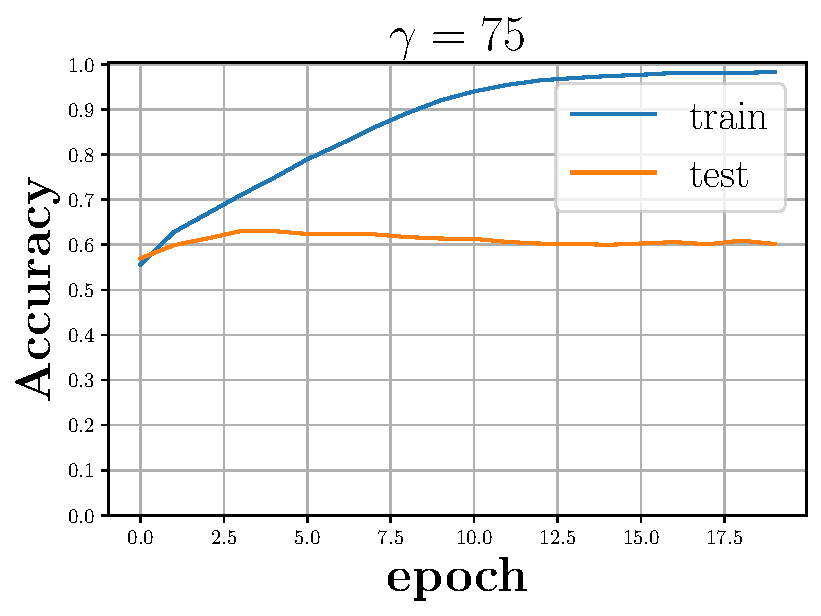
\includegraphics[scale=0.125]{figs/galu_75_good.pdf}&
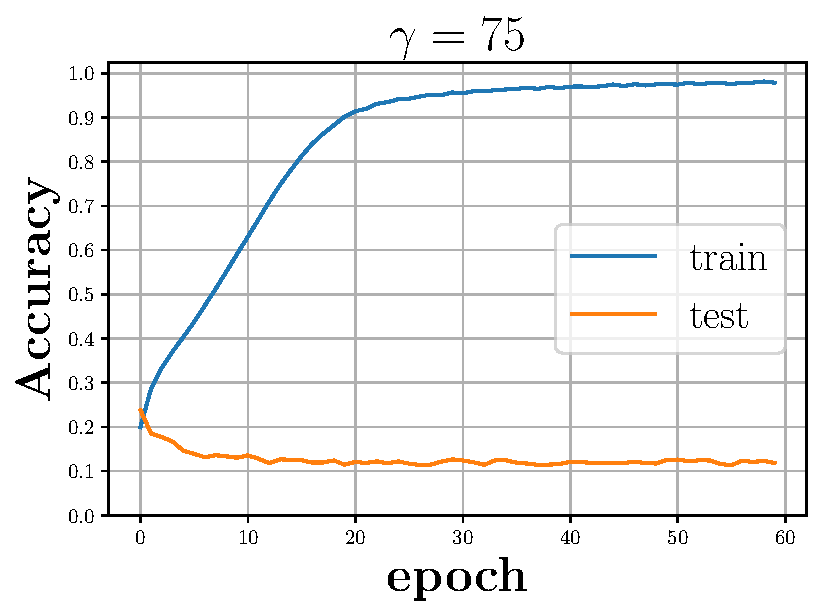
\includegraphics[scale=0.125]{figs/galu_75_bad.pdf}&
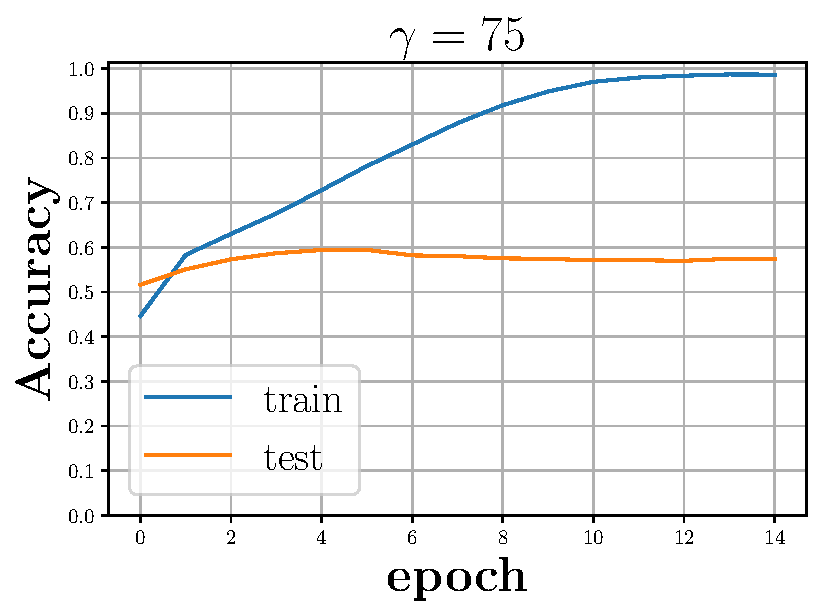
\includegraphics[scale=0.125]{figs/galu_75_bad_good.pdf}&
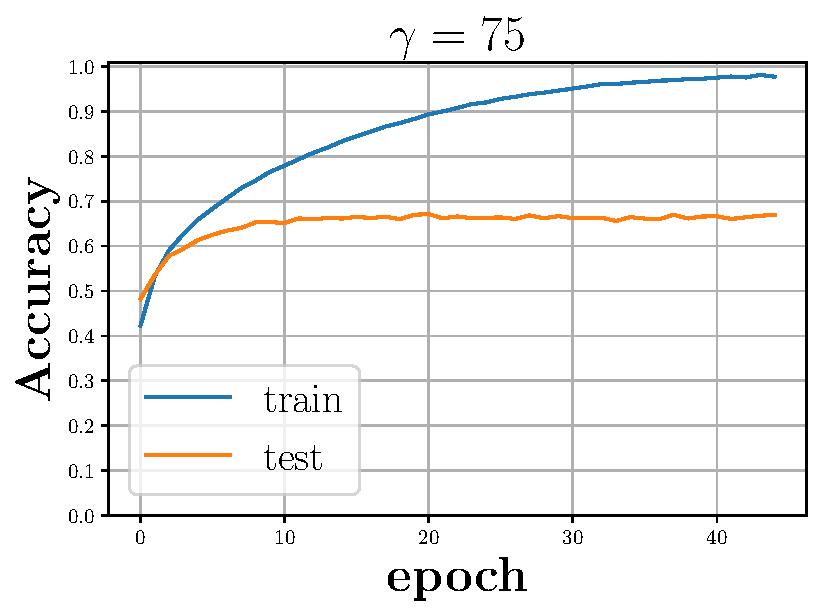
\includegraphics[scale=0.125]{figs/relu_75_good.pdf}&
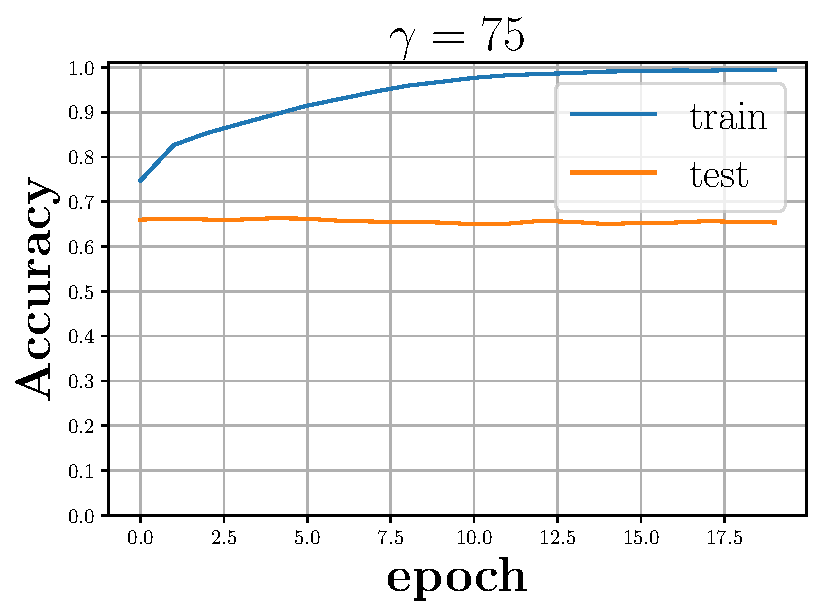
\includegraphics[scale=0.125]{figs/galu_75_recovered.pdf}\\
\tiny{M1}&\tiny{M2}&\tiny{M3:US}&\tiny{M3:DS}&\tiny{M4}&\tiny{M5}\\
\end{tabular}
}
\end{minipage}

\label{fig:rand-label}

\end{figure}

\end{comment}


\begin{comment}
\begin{figure}[h]
\begin{minipage}{0.40\columnwidth}
\begin{tabular}{|c|c|c|}\hline
ReLU& \multicolumn{2}{c|}{}\\
with   & \multicolumn{2}{c|}{Fixed Learnt Gates from }\\
 True &\multicolumn{2}{c|}{ReLU with True Labels}\\
Labels &  \multicolumn{2}{c|}{}\\\cline{2-3}
&True & {US/DS}\\\hline
 80.8& 80& 79\\\hline
 col-1 & col-2 & col-3\\\hline
\end{tabular}

\end{minipage}
\begin{minipage}{0.62\columnwidth}
\begin{tabular}{|c|c|c|c|c|c|c|c|}\hline
\%& \multicolumn{3}{c|}{\multirow{2}{*}{ReLU}} & \multicolumn{2}{c|}{FLG at End}&{FLG at End}\\
Label& \multicolumn{3}{c|}{{}} &\multicolumn{2}{c|}{of ReLU US}& of ReLU DS\\\cline{2-7}
Noise & \multicolumn{2}{c|}{Rand. US} & True & \multicolumn{1}{c|}{\multirow{2}{*}{True}} &{US/DS}& \multicolumn{1}{c|}{\multirow{2}{*}{True}} \\\cline{2-3}
{} & Best & End & DS &{} &  &\\\hline
25&75.3 & 63.1& 76.7&74.2 & 72.3& 76.5\\\hline
50& 69.8 &41.5&73.1&69.6 &67& 73.1\\\hline
 col-1 & col-2 & col-3&  col-4 & col-5 & col-6& col-7\\\hline
\end{tabular}
\end{minipage}
\end{figure}
\end{comment}

